% Options for packages loaded elsewhere
\PassOptionsToPackage{unicode}{hyperref}
\PassOptionsToPackage{hyphens}{url}
%
\documentclass[
  english,
]{book}
\usepackage{amsmath,amssymb}
\usepackage{lmodern}
\usepackage{ifxetex,ifluatex}
\ifnum 0\ifxetex 1\fi\ifluatex 1\fi=0 % if pdftex
  \usepackage[T1]{fontenc}
  \usepackage[utf8]{inputenc}
  \usepackage{textcomp} % provide euro and other symbols
\else % if luatex or xetex
  \usepackage{unicode-math}
  \defaultfontfeatures{Scale=MatchLowercase}
  \defaultfontfeatures[\rmfamily]{Ligatures=TeX,Scale=1}
\fi
% Use upquote if available, for straight quotes in verbatim environments
\IfFileExists{upquote.sty}{\usepackage{upquote}}{}
\IfFileExists{microtype.sty}{% use microtype if available
  \usepackage[]{microtype}
  \UseMicrotypeSet[protrusion]{basicmath} % disable protrusion for tt fonts
}{}
\makeatletter
\@ifundefined{KOMAClassName}{% if non-KOMA class
  \IfFileExists{parskip.sty}{%
    \usepackage{parskip}
  }{% else
    \setlength{\parindent}{0pt}
    \setlength{\parskip}{6pt plus 2pt minus 1pt}}
}{% if KOMA class
  \KOMAoptions{parskip=half}}
\makeatother
\usepackage{xcolor}
\IfFileExists{xurl.sty}{\usepackage{xurl}}{} % add URL line breaks if available
\IfFileExists{bookmark.sty}{\usepackage{bookmark}}{\usepackage{hyperref}}
\hypersetup{
  pdftitle={ReCentering Psych Stats: Analysis of Variance},
  pdfauthor={Lynette H Bikos, PhD, ABPP},
  pdflang={en},
  hidelinks,
  pdfcreator={LaTeX via pandoc}}
\urlstyle{same} % disable monospaced font for URLs
\usepackage{color}
\usepackage{fancyvrb}
\newcommand{\VerbBar}{|}
\newcommand{\VERB}{\Verb[commandchars=\\\{\}]}
\DefineVerbatimEnvironment{Highlighting}{Verbatim}{commandchars=\\\{\}}
% Add ',fontsize=\small' for more characters per line
\usepackage{framed}
\definecolor{shadecolor}{RGB}{248,248,248}
\newenvironment{Shaded}{\begin{snugshade}}{\end{snugshade}}
\newcommand{\AlertTok}[1]{\textcolor[rgb]{0.94,0.16,0.16}{#1}}
\newcommand{\AnnotationTok}[1]{\textcolor[rgb]{0.56,0.35,0.01}{\textbf{\textit{#1}}}}
\newcommand{\AttributeTok}[1]{\textcolor[rgb]{0.77,0.63,0.00}{#1}}
\newcommand{\BaseNTok}[1]{\textcolor[rgb]{0.00,0.00,0.81}{#1}}
\newcommand{\BuiltInTok}[1]{#1}
\newcommand{\CharTok}[1]{\textcolor[rgb]{0.31,0.60,0.02}{#1}}
\newcommand{\CommentTok}[1]{\textcolor[rgb]{0.56,0.35,0.01}{\textit{#1}}}
\newcommand{\CommentVarTok}[1]{\textcolor[rgb]{0.56,0.35,0.01}{\textbf{\textit{#1}}}}
\newcommand{\ConstantTok}[1]{\textcolor[rgb]{0.00,0.00,0.00}{#1}}
\newcommand{\ControlFlowTok}[1]{\textcolor[rgb]{0.13,0.29,0.53}{\textbf{#1}}}
\newcommand{\DataTypeTok}[1]{\textcolor[rgb]{0.13,0.29,0.53}{#1}}
\newcommand{\DecValTok}[1]{\textcolor[rgb]{0.00,0.00,0.81}{#1}}
\newcommand{\DocumentationTok}[1]{\textcolor[rgb]{0.56,0.35,0.01}{\textbf{\textit{#1}}}}
\newcommand{\ErrorTok}[1]{\textcolor[rgb]{0.64,0.00,0.00}{\textbf{#1}}}
\newcommand{\ExtensionTok}[1]{#1}
\newcommand{\FloatTok}[1]{\textcolor[rgb]{0.00,0.00,0.81}{#1}}
\newcommand{\FunctionTok}[1]{\textcolor[rgb]{0.00,0.00,0.00}{#1}}
\newcommand{\ImportTok}[1]{#1}
\newcommand{\InformationTok}[1]{\textcolor[rgb]{0.56,0.35,0.01}{\textbf{\textit{#1}}}}
\newcommand{\KeywordTok}[1]{\textcolor[rgb]{0.13,0.29,0.53}{\textbf{#1}}}
\newcommand{\NormalTok}[1]{#1}
\newcommand{\OperatorTok}[1]{\textcolor[rgb]{0.81,0.36,0.00}{\textbf{#1}}}
\newcommand{\OtherTok}[1]{\textcolor[rgb]{0.56,0.35,0.01}{#1}}
\newcommand{\PreprocessorTok}[1]{\textcolor[rgb]{0.56,0.35,0.01}{\textit{#1}}}
\newcommand{\RegionMarkerTok}[1]{#1}
\newcommand{\SpecialCharTok}[1]{\textcolor[rgb]{0.00,0.00,0.00}{#1}}
\newcommand{\SpecialStringTok}[1]{\textcolor[rgb]{0.31,0.60,0.02}{#1}}
\newcommand{\StringTok}[1]{\textcolor[rgb]{0.31,0.60,0.02}{#1}}
\newcommand{\VariableTok}[1]{\textcolor[rgb]{0.00,0.00,0.00}{#1}}
\newcommand{\VerbatimStringTok}[1]{\textcolor[rgb]{0.31,0.60,0.02}{#1}}
\newcommand{\WarningTok}[1]{\textcolor[rgb]{0.56,0.35,0.01}{\textbf{\textit{#1}}}}
\usepackage{longtable,booktabs,array}
\usepackage{calc} % for calculating minipage widths
% Correct order of tables after \paragraph or \subparagraph
\usepackage{etoolbox}
\makeatletter
\patchcmd\longtable{\par}{\if@noskipsec\mbox{}\fi\par}{}{}
\makeatother
% Allow footnotes in longtable head/foot
\IfFileExists{footnotehyper.sty}{\usepackage{footnotehyper}}{\usepackage{footnote}}
\makesavenoteenv{longtable}
\usepackage{graphicx}
\makeatletter
\def\maxwidth{\ifdim\Gin@nat@width>\linewidth\linewidth\else\Gin@nat@width\fi}
\def\maxheight{\ifdim\Gin@nat@height>\textheight\textheight\else\Gin@nat@height\fi}
\makeatother
% Scale images if necessary, so that they will not overflow the page
% margins by default, and it is still possible to overwrite the defaults
% using explicit options in \includegraphics[width, height, ...]{}
\setkeys{Gin}{width=\maxwidth,height=\maxheight,keepaspectratio}
% Set default figure placement to htbp
\makeatletter
\def\fps@figure{htbp}
\makeatother
\setlength{\emergencystretch}{3em} % prevent overfull lines
\providecommand{\tightlist}{%
  \setlength{\itemsep}{0pt}\setlength{\parskip}{0pt}}
\setcounter{secnumdepth}{5}
\usepackage{booktabs}
\ifxetex
  % Load polyglossia as late as possible: uses bidi with RTL langages (e.g. Hebrew, Arabic)
  \usepackage{polyglossia}
  \setmainlanguage[]{english}
\else
  \usepackage[main=english]{babel}
% get rid of language-specific shorthands (see #6817):
\let\LanguageShortHands\languageshorthands
\def\languageshorthands#1{}
\fi
\ifluatex
  \usepackage{selnolig}  % disable illegal ligatures
\fi
\usepackage[]{natbib}
\bibliographystyle{plainnat}

\title{ReCentering Psych Stats: Analysis of Variance}
\author{Lynette H Bikos, PhD, ABPP}
\date{}

\begin{document}
\maketitle

{
\setcounter{tocdepth}{1}
\tableofcontents
}
\hypertarget{book-cover}{%
\chapter*{BOOK COVER}\label{book-cover}}
\addcontentsline{toc}{chapter}{BOOK COVER}

\begin{figure}
\centering
\includegraphics{images/ReC_ANOVA_bookcover.png}
\caption{An image of the book cover. It includes four quadrants of non-normal distributions representing gender, race/ethnicty, sustainability/global concerns, and journal articles}
\end{figure}

\hypertarget{preface}{%
\chapter*{Preface}\label{preface}}
\addcontentsline{toc}{chapter}{Preface}

\textbf{If you are viewing this document, you should know that this is a book-in-progress. Early drafts are released for the purpose teaching my classes and gaining formative feedback from a host of stakeholders. The document was last updated on 07 Aug 2021}

\href{https://spu.hosted.panopto.com/Panopto/Pages/Viewer.aspx?id=c932455e-ef06-444a-bdca-acf7012d759a}{Screencasted Lecture Link}

To \emph{center} a variable in regression means to set its value at zero and interpret all other values in relation to this reference point. Regarding race and gender, researchers often center male and White at zero. Further, it is typical that research vignettes in statistics textbooks are similarly seated in a White, Western (frequently U.S.), heteronormative, framework. The purpose of this project is to create a set of open educational resources (OER) appropriate for doctoral and post-doctoral training that contribute to a socially responsive pedagogy -- that is, it contributes to justice, equity, diversity, and inclusion.

Statistics training in doctoral programs are frequently taught with fee-for-use programs (e.g., SPSS/AMOS, SAS, MPlus) that may not be readily available to the post-doctoral professional. In recent years, there has been an increase and improvement in R packages (e.g., \emph{psych}, \emph{lavaan}) used for in analyses common to psychological research. Correspondingly, many graduate programs are transitioning to statistics training in R (free and open source). This is a challenge for post-doctoral psychologists who were trained with other software. This OER will offer statistics training with R and be freely available (specifically in a GitHub respository and posted through GitHub Pages) under a Creative Commons Attribution - Non Commercial - Share Alike license {[}CC BY-NC-SA 4.0{]}.

Training models for doctoral programs in HSP are commonly scholar-practitioner, scientist-practitioner, or clinical-scientist. An emerging model, the \emph{scientist-practitioner-advocacy} training model incorporates social justice advocacy so that graduates are equipped to recognize and address the sociocultural context of oppression and unjust distribution of resources and opportunities \citep{mallinckrodt_scientist-practitioner-advocate_2014}. In statistics textbooks, the use of research vignettes engages the learner around a tangible scenario for identifying independent variables, dependent variables, covariates, and potential mechanisms of change. Many students recall examples in Field's \citeyearpar{field_discovering_2012} popular statistics text: Viagra to teach one-way ANOVA, beer goggles for two-way ANOVA, and bushtucker for repeated measures. What if the research vignettes were more socially responsive?

In this OER, research vignettes will be from recently published articles where:

\begin{itemize}
\tightlist
\item
  the author's identity is from a group where scholarship is historically marginalized (e.g., BIPOC, LGBTQ+, LMIC{[}low-middle income countries{]}),
\item
  the research is responsive to issues of justice, equity, inclusion, diversity,
\item
  the lesson's statistic is used in the article, and
\item
  there is sufficient information in the article to simulate the data for the chapter example(s) and practice problem(s); or it is publicly available.
\end{itemize}

In training for multicultural competence, the saying, ``A fish doesn't know that it's wet'' is often used to convey the notion that we are often unaware of our own cultural characteristics. In recent months and years, there has been an increased awakening to the institutional and systemic racism that our systems are perpetuating. Queuing from the water metaphor, I am hopeful that a text that is recentered in the ways I have described can contribute to \emph{changing the water} in higher education and in the profession of psychology.

\hypertarget{copyright-with-open-access}{%
\section*{Copyright with Open Access}\label{copyright-with-open-access}}
\addcontentsline{toc}{section}{Copyright with Open Access}

This book is published under a a Creative Commons Attribution-NonCommercial-ShareAlike 4.0 International License. This means that this book can be reused, remixed, retained, revised and redistributed (including commercially) as long as appropriate credit is given to the authors. If you remix, or modify the original version of this open textbook, you must redistribute all versions of this open textbook under the same license - CC BY-SA.

A \href{https://github.com/lhbikos/ReCenterPsychStats}{GitHub open-source repository} contains all of the text and source code for the book, including data and images.

\hypertarget{acknowledgements}{%
\chapter*{ACKNOWLEDGEMENTS}\label{acknowledgements}}
\addcontentsline{toc}{chapter}{ACKNOWLEDGEMENTS}

As a doctoral student at the University of Kansas (1992-2005), I learned that ``a foreign language'' was required for graduation. \emph{Please note that as one who studies the intersections of global, vocational, and sustainable psychology, I regret that I do not have language skills beyond English.} This could have been met with credit from high school my rural, mid-Missouri high school did not offer such classes. This requirement would have typically been met with courses taken during an undergraduate program -- but my non-teaching degree in the University of Missouri's School of Education was exempt from this. The requirement could have also been met with a computer language (fortran, C++) -- I did not have any of those either. There was a tiny footnote on my doctoral degree plan that indicated that a 2-credit course, ``SPSS for Windows'' would substitute for the language requirement. Given that it was taught by my one of my favorite professors, I readily signed up. As it turns out, Samuel B. Green, PhD, was using the course to draft chapters in the textbook \citep{green_using_2014} that has been so helpful for so many. Unfortunately, Drs. Green (1947 - 2018) and Salkind (2947 - 2017) are no longer with us. I have worn out numerous versions of their text. Another favorite text of mine was Dr.~Barbara Byrne's \citeyearpar{byrne_structural_2016}, ``Structural Equation Modeling with AMOS.'' I loved the way she worked through each problem and paired it with a published journal article, so that the user could see how the statistical evaluation fit within the larger project/article. I took my tea-stained text with me to a workshop she taught at APA and was proud of the signature she added to it (a little catfur might have fallen out). Dr.~Byrne created SEM texts for a number of statistical programs (e.g., LISREL, EQS, MPlus). As I was learning R, I wrote Dr.~Byrne, asking if she had an edition teaching SEM/CFA with R. She promptly wrote back, saying that she did not have the bandwidth to learn a new statistics package. We lost Dr.~Byrne in December 2020. I am so grateful to these role models for their contributions to my statistical training. I am also grateful for the doctoral students who have taken my courses and are continuing to provide input for how to improve the materials.

The inspiration for training materials that re*center statistics and research methods came from the \href{https://www.academics4blacklives.com/}{Academics for Black Survival and Wellness Initiative}. This project, co-founded by Della V. Mosley, Ph.D., and Pearis L. Bellamy, M.S., made clear the necessity and urgency for change in higher education and the profession of psychology.

At very practical levels, I am indebted to SPU's Library, and more specifically, SPU's Education, Technology, and Media Department. Assistant Dean for Instructional Design and Emerging Technologies, R. John Robertson, MSc, MCS, has offered unlimited consultation, support, and connection. Senior Instructional Designer in Graphics \& Illustrations, Dominic Wilkinson, designed the logo and bookcover. Psychology and Scholarly Communications Librarian, Kristin Hoffman, MLIS, has provided consultation on topics ranging from OERS to citations. I am alo indebted to Associate Vice President, Teaching and Learning at Kwantlen Polytechnic University, Rajiv Jhangiani, PhD. Dr.~Jhangiani's text \citeyearpar{jhangiani_research_2019} was the first OER I ever used and I was grateful for his encouraging conversation.

Financial support for this text has been provided from the \emph{Call to Action on Equity, Inclusion, Diversity, Justice, and Social Responsivity
Request for Proposals} grant from the Association of Psychology Postdoctoral and Internship Centers (2021-2022).

\hypertarget{ReCintro}{%
\chapter{Introduction}\label{ReCintro}}

\href{https://spu.hosted.panopto.com/Panopto/Pages/Viewer.aspx?pid=cc9b7c0d-e5c3-4e4e-a469-acf7013ee761}{Screencasted Lecture Link}

\hypertarget{what-to-expect-in-each-chapter}{%
\section{What to expect in each chapter}\label{what-to-expect-in-each-chapter}}

This textbook is intended as \emph{applied,} in that a primary goal is to help the scientist-practitioner-advocate use a variety of statistics in research problems and \emph{writing them up} for a program evaluation, dissertation, or journal article. In support of that goal, I try to provide just enough conceptual information so that the researcher can select the appropriate statistic (i.e., distinguishing between when ANOVA is appropriate and when regression is appropriate) and assign variables to their proper role (e.g., covariate, moderator, mediator).

This conceptual approach does include occasional, step-by-step, \emph{hand-calculations} (only we calculate them arithmetically in R) to provide a \emph{visceral feeling} of what is happening within the statistical algorithm that may be invisible to the researcher. Additionally, the conceptual review includes a review of the assumptions about the characteristics of the data and research design that are required for the statistic. Statistics can be daunting, so I have worked hard to establish a \emph{workflow} through each analysis. When possible, I include a flowchart that is referenced frequently in each chapter and assists the the researcher keep track of their place in the many steps and choices that accompany even the simplest of analyses.

As with many statistics texts, each chapter includes a \emph{research vignette.} Somewhat unique to this resource is that the vignettes are selected from recently published articles. Each vignette is chosen with the intent to meet as many of the following criteria as possible:

\begin{itemize}
\tightlist
\item
  the statistic that is the focus of the chapter was properly used in the article,
\item
  the author's identity is from a group where scholarship is historically marginalized (e.g., BIPOC, LGBTQ+, LMIC {[}low middle income countries{]}),
\item
  the research has a justice, equity, inclusion, diversity, and social responsivity focus and will contribute positively to a social justice pedagogy, and
\item
  the data is available in a repository or there is sufficient information in the article to simulate the data for the chapter example(s) and practice problem(s).
\end{itemize}

In each chapter we employ \emph{R} packages that will efficiently calculate the statistic and the dashboard of metrics (e.g., effect sizes, confidence intervals) that are typically reported in psychological science.

\hypertarget{strategies-for-accessing-and-using-this-oer}{%
\section{Strategies for Accessing and Using this OER}\label{strategies-for-accessing-and-using-this-oer}}

There are a number of ways you can access this resource. You may wish to try several strategies and then select which works best for you. I demonstrate these in the screencast that accompanies this chapter.

\begin{enumerate}
\def\labelenumi{\arabic{enumi}.}
\tightlist
\item
  Simply follow along in the .html formatted document that is available on via GitHug Pages, and then

  \begin{itemize}
  \tightlist
  \item
    open a fresh .rmd file of your own, copying (or retyping) the script and running it
  \end{itemize}
\item
  Locate the original documents at the \href{https://github.com/lhbikos/ReCenterPsychStats}{GitHub repository} . You can

  \begin{itemize}
  \tightlist
  \item
    open them to simply take note of the ``behind the scenes'' script
  \item
    copy/download individual documents that are of interest to you
  \item
    fork a copy of the entire project to your own GitHub site and further download it (in its entirety) to your personal workspace. The \href{https://desktop.github.com/}{GitHub Desktop app} makes this easy!
  \end{itemize}
\item
  Listen to the accompanying lectures (I think sound best when the speed is 1.75). The lectures are being recorded in Panopto and should include the closed captioning.
\item
  Provide feedback to me! If you fork a copy to your own GitHub repository, you can

  \begin{itemize}
  \tightlist
  \item
    open up an editing tool and mark up the document with your edits,
  \item
    start a discussion by leaving comments/questions, and then
  \item
    sending them back to me by committing and saving. I get an e-mail notiying me of this action. I can then review (accepting or rejecting) them and, if a discussion is appropriate, reply back to you.
  \end{itemize}
\end{enumerate}

\hypertarget{if-you-are-new-to-r}{%
\section{If You are New to R}\label{if-you-are-new-to-r}}

R can be oveRwhelming. Jumping right into advanced statistics might not be the easiest way to start. However, in these chapters, I provide complete code for every step of the process, starting with uploading the data. To help explain what R script is doing, I sometimes write it in the chapter text; sometimes leave hastagged-comments in the chunks; and, particularly in the accompanying screencasted lectures, try to take time to narrate what the R script is doing.

I've found that, somewhere on the internet, there's almost always a solution to what I'm trying to do. I am frequently stuck and stumped and have spent hours searching the internet for even the tiniest of things. When you watch my videos, you may notice that in my R studio, there is a ``scRiptuRe'' file. I takes notes on the solutions and scripts here -- using keywords that are meaningful to me so that when I need to repeat the task, I can hopefully search my own prior solutions and find a fix or a hint.

\hypertarget{base-r}{%
\subsection{Base R}\label{base-r}}

The base program is free and is available here: \url{https://www.r-project.org/}

Because R is already on my machine (and because the instructions are sufficient), I will not walk through the instllation, but I will point out a few things.

\begin{itemize}
\tightlist
\item
  Follow the instructions for your operating system (Mac, Windows, Linux)
\item
  The ``cran'' (I think ``cranium'') is the \emph{Comprehensive R Archive Network.} In order for R to run on your computer, you have to choose a location. Because proximity is somewhat related to processing speed, select one that is geographically ``close to you.''
\item
  You will see the results of this download on your desktop (or elsewhere if you chose to not have it appear there) but you won't ever use R through this platform.
\end{itemize}

\hypertarget{r-studio}{%
\subsection{R Studio}\label{r-studio}}

\emph{R Studio} is the desktop application I work in R. It's a separate download. Choose the free, desktop, option that is appropriate for your operating system: \url{https://www.rstudio.com/products/RStudio/}

\begin{itemize}
\tightlist
\item
  Upper right window: Includes several tabs; we frequently monitor the

  \begin{itemize}
  \tightlist
  \item
    Environment: it lists the \emph{objects} that are available to you (e.g., dataframes)
  \end{itemize}
\item
  Lower right window: has a number of helpful tabs.

  \begin{itemize}
  \tightlist
  \item
    Files: Displays the file structure in your computer's environment. Make it a practice to (a) organize your work in small folders and (b) navigating to that small folder that is holding your project when you are working on it.
  \item
    Packages: Lists the packages that have been installed. If you navigate to it, you can see if it is ``on.'' You can also access information about the package (e.g., available functions, examples of script used with the package) in this menu. This information opens in the Help window.
  \item
    Viewer and Plots are helpful, later, when we can simultaneously look at our output and still work on our script.
  \end{itemize}
\item
  Primary window

  \begin{itemize}
  \tightlist
  \item
    R Studio runs in the background(in the console). Very occasionally, I can find useful troubleshooting information here.
  \item
    More commonly, I open my R Markdown document so that it takes the whole screen and I work directly, right here.
  \end{itemize}
\item
  \emph{R Markdown} is the way that many analysts write \emph{script}, conduct analyses, and even write up results. These are saved as .rmd files.

  \begin{itemize}
  \tightlist
  \item
    In R Studio, open an R Markdown document through File/New File/R Markdown
  \item
    Specify the details of your document (title, author, desired ouput)
  \item
    In a separate step, SAVE this document (File/Save{]} into a NEW FILE FOLDER that will contain anything else you need for your project (e.g., the data).
  \item
    \emph{Packages} are at the heart of working in R. Installing and activating packages require writing script.
  \end{itemize}
\end{itemize}

\hypertarget{r-hygiene}{%
\subsection{R Hygiene}\label{r-hygiene}}

Many initial problems in R can be solved with good R hygiene. Here are some suggestions for basic practices. It can be tempting to ``skip this.'' However, in the first few weeks of class, these are the solutions I am presenting to my students.

\hypertarget{everything-is-documented-in-the-.rmd-file}{%
\subsubsection{Everything is documented in the .rmd file}\label{everything-is-documented-in-the-.rmd-file}}

Although others do it differently, everything is in my .rmd file. That is, for uploading data and opening packages I write the code in my .rmd file. Why? Because when I read about what I did hours or years later, I have a permanent record of very critical things like (a) where my data is located, (b) what version I was using, and (c) what package was associated with the functions.

\hypertarget{file-organization}{%
\subsubsection{File organization}\label{file-organization}}

File organization is a critical key to this:

\begin{itemize}
\tightlist
\item
  Create a project file folder.
\item
  Put the data file in it.
\item
  Open an R Markdown file.
\item
  Save it in the same file folder.
\item
  When your data and .rmd files are in the same folder (not your desktop, but a shared folder), they can be connected.
\end{itemize}

\hypertarget{chunks}{%
\subsubsection{Chunks}\label{chunks}}

The R Markdown document is an incredible tool for integrating text, tables, and analyses. This entire OER is written in R Markdown. A central feature of this is ``chunks.''

The easiest way to insert a chunk is to use the INSERT/R command at the top of this editor box. You can also insert a chunk with the keyboard shortcut: CTRL/ALT/i

``Chunks'' start and end with with those three tic marks and will show up in a shaded box, like this:

\begin{Shaded}
\begin{Highlighting}[]
\CommentTok{\#hashtags let me write comments to remind myself what I did}
\CommentTok{\#here I am simply demonstrating arithmetic (but I would normally be running code)}
\DecValTok{2021} \SpecialCharTok{{-}} \DecValTok{1966}
\end{Highlighting}
\end{Shaded}

\begin{verbatim}
## [1] 55
\end{verbatim}

Each chunk must open and close. If one or more of your tic marks get deleted, your chunk won't be read as such and your script will not run. The only thing in the chunks should be script for running R; you can hashtag-out script so it won't run.

Although unnecessary, you can add a brief title for the chunk in the opening row, after the ``r.'' These create something of a table of contents of all the chunks -- making it easier to find what you did. You can access them in the ``Chunks'' tab at the bottom left of R Studio. If you wish to knit a document, you cannot have identical chunk titles.

You can put almost anything you want in the space outside of tics. Syntax for simple formatting in the text areas (e.g,. using italics, making headings, bold, etc.) is found here: \url{https://rmarkdown.rstudio.com/authoring_basics.html}

\hypertarget{packages}{%
\subsubsection{Packages}\label{packages}}

As scientist-practitioners (and not coders), we will rely on \emph{packages} to do our work for us. At first you may feel overwhelmed about the large number of packages that are available. Soon, though, you will become accustomed to the ones most applicable to our work (e.g., psych, tidyverse, lavaan, apaTables).

Researchers treat packages differently. In these lectures, I list all the packages we will use in an opening chunk that asks R to check to see if the package is installed, and if not, installs it.

\begin{Shaded}
\begin{Highlighting}[]
\ControlFlowTok{if}\NormalTok{(}\SpecialCharTok{!}\FunctionTok{require}\NormalTok{(psych))\{}\FunctionTok{install.packages}\NormalTok{(}\StringTok{"psych"}\NormalTok{)\}}
\end{Highlighting}
\end{Shaded}

\begin{verbatim}
## Loading required package: psych
\end{verbatim}

\begin{verbatim}
## Warning: package 'psych' was built under R version 4.0.5
\end{verbatim}

To make a package operable, you need to open it through the library. This process must be repeated each time you restart R. I don't open the package (through the ``library(package\_name)'') command until it is time to use it. Especially for new users, I think it's important to connect the functions with the specific packages.

\begin{Shaded}
\begin{Highlighting}[]
\CommentTok{\#install.packages ("psych")}
\FunctionTok{library}\NormalTok{ (psych)}
\end{Highlighting}
\end{Shaded}

If you type in your own ``install.packages'' code, hashtag it out once it's been installed. It is problematic to continue to re-run this code .

\hypertarget{knitting}{%
\subsubsection{Knitting}\label{knitting}}

An incredible feature of R Markdown is its capacity to \emph{knit} to HTML, powerpoint, or word. If you access the .rmd files for this OER, you can use annotate or revise them to suit your purposes. If you redistribute them, though, please honor the Creative Commons Attribution-NonCommercial-ShareAlike 4.0 International License with a citation.

\hypertarget{troubleshooting-in-r-markdown}{%
\subsection{tRoubleshooting in R maRkdown}\label{troubleshooting-in-r-markdown}}

Hiccups are normal. Here are some ideas that I have found useful in getting unstuck.

\begin{itemize}
\tightlist
\item
  In an R script, you must have everything in order -- Every. Single. Time.

  \begin{itemize}
  \tightlist
  \item
    All the packages have to be in your library and activated; if you restart R, you need to reload each package.
  \item
    If you open an .rmd file and want a boxplot, you cannot just scroll down to that script. You need to run any \emph{prerequisite} script (like loading the package, importing data, putting the data in the global environment, etc.)
  \item
    Do you feel lost? clear your global environment (broom) and start at the top of the R script. Frequent, fresh starts are good.
  \end{itemize}
\item
  Your .rmd file and your data need to be stored in the same file folder. These should be separate for separate projects, no matter how small.
\item
  Type any warnings you get into a search engine. Odds are, you'll get some decent hints in a manner of seconds. Especially at first, these are common errors:

  \begin{itemize}
  \tightlist
  \item
    The package isn't loaded (if you restarted R, you need to reload your packages)
  \item
    The .rmd file has been saved yet, or isn't saved in the same folder as the data
  \item
    Errors of punctuation or spelling
  \end{itemize}
\item
  Restart R (it's quick -- not like restarting your computer)
\item
  If you receive an error indicating that a function isn't working or recognized, and you have loaded the package, type the name of the package in front of the function with two colons (e.g., psych::describe(df). If multiple packages are loaded with functions that have the same name, R can get confused.
\end{itemize}

\hypertarget{strategies-for-success}{%
\subsection{stRategies for success}\label{strategies-for-success}}

\begin{itemize}
\tightlist
\item
  Engage with R, but don't let it overwhelm you.

  \begin{itemize}
  \tightlist
  \item
    The \emph{mechanical is also the conceptual}. Especially when it is \emph{simpler}, do try to retype the script into your own .rmd file and run it. Track down the errors you are making and fix them.
  \item
    If this stresses you out, move to simply copying the code into the .rmd file and running it. If you continue to have errors, you may have violated one of the best practices above (Is the package loaded? Are the data and .rmd files in the same place? Is all the prerequisite script run?).
  \item
    Still overwhelmed? Keep moving forward by downloading a copy of the .rmd file that accompanies any given chapter and just ``run it along'' with the lecture. Spend your mental power trying to understand what each piece does. Then select a practice problem that is appropriate for your next level of growth.
  \end{itemize}
\item
  Copy script that works elsewhere and replace it with your datafile, variables, etc.\\
\item
  The leaRning curve is steep, but not impossible. Gladwell\citeyearpar{gladwell_outliers_2008} reminds us that it takes about 10,000 hours to get GREAT at something (2,000 to get reasonably competent). Practice. Practice. Practice.
\item
  Updates to R, R Studio, and the packages are NECESSARY, but can also be problematic. It could very well be that updates cause programs/script to fail (e.g., ``X has been deprecated for version X.XX''). Moreover, this very well could have happened between my distribution of these resources and your attempt to use it. My personal practice is to update R, R Studio, and the packages a week or two before each academic term.
\item
  Embrace your downward dog. Also, walk away, then come back.
\end{itemize}

\hypertarget{resources-for-getting-started}{%
\subsection{Resources for getting staRted}\label{resources-for-getting-started}}

R for Data Science: \url{https://r4ds.had.co.nz/}

R Cookbook: \url{http://shop.oreilly.com/product/9780596809164.do}

R Markdown homepage with tutorials: \url{https://rmarkdown.rstudio.com/index.html}

R has cheatsheets for everything, here's one for R Markdown: \url{https://www.rstudio.com/wp-content/uploads/2015/02/rmarkdown-cheatsheet.pdf}

R Markdown Reference guide: \url{https://www.rstudio.com/wp-content/uploads/2015/03/rmarkdown-reference.pdf}

Using R Markdown for writing reproducible scientific papers: \url{https://libscie.github.io/rmarkdown-workshop/handout.html}

LaTeX equation editor: \url{https://www.codecogs.com/latex/eqneditor.php}

\hypertarget{Ready}{%
\chapter{Ready\_Set\_R}\label{Ready}}

\href{https://spu.hosted.panopto.com/Panopto/Pages/Viewer.aspx?id=d080e0bb-e52e-4f38-9965-aa67010b3567}{Screencasted Lecture Link}

With the goal of creating a common, system-wide approach to using the platorm, this lesson is primarily created for CPY and I/O doctoral students who are entering the ``stats sequence.''I hope it will also be useful for others (including faculty) who are also making the transition to R.

\hypertarget{navigating-this-lesson}{%
\section{Navigating this Lesson}\label{navigating-this-lesson}}

There is about 45 minutes of lecture.

\hypertarget{learning-objectives}{%
\subsection{Learning Objectives}\label{learning-objectives}}

Learning objectives from this lecture include the following:

\begin{itemize}
\tightlist
\item
  Downloading/installing R's parts and pieces.
\item
  Using R-Markdown as the interface for running R analyses and saving the script.
\item
  Recognizing and adopting best practices for ``R hygiene.''
\item
  Identifying effective strategies for troubleshooting R hiccups.
\end{itemize}

\hypertarget{downloading-and-installing-r}{%
\section{downloading and installing R}\label{downloading-and-installing-r}}

\hypertarget{so-many-parts-and-pieces}{%
\subsection{So many paRts and pieces}\label{so-many-parts-and-pieces}}

Before we download, it may be helpful to understand some of R's many parts and pieces.

The base software is free and is available \href{https://www.r-project.org/}{here}

Because R is already on my machine (and because the instructions are sufficient), I will not walk through the demo, but I will point out a few things.

\begin{itemize}
\tightlist
\item
  The ``cran'' (I think ``cranium'') is the \emph{Comprehensive R Archive Network.} In order for R to run on your computer, you have to choose a location -- and it should be geographically ``close to you.''

  \begin{itemize}
  \tightlist
  \item
    Follow the instructions for your operating system (Mac, Windows, Linux)
  \item
    You will see the results of this download on your desktop (or elsewhere if you chose to not have it appear there) but you won't ever use R through this platform.
  \end{itemize}
\item
  \href{https://www.rstudio.com/products/RStudio/}{R Studio} is the way in which we operate R. It's a separate download. Choose the free, desktop, option that is appropriate for your operating system:\\
\item
  \emph{R Markdown} is the way that many analysts write \emph{script}, conduct analyses, and even write up results. These are saved as .rmd files.

  \begin{itemize}
  \tightlist
  \item
    In R Studio, open an R Markdown document through File/New File/R Markdown
  \item
    Specify the details of your document (title, author, desired ouput)
  \item
    In a separate step, SAVE this document (File/Save{]} into a NEW FILE FOLDER that will contain anything else you need for your project (e.g., the data).
  \item
    \emph{Packages} are at the heart of working in R. Installing and activating packages require writing script.
  \end{itemize}
\end{itemize}

\textbf{Note} If you have an enterprise-owned machine (e.g,. in my specific context, if you are a faculty/staff or have a lab with an SPU-issued laptops) there are complications caused by how documents are stored. You will likely need to consult with your computer and technology support office.

\hypertarget{orienting-to-r-studio-focusing-only-on-the-things-we-will-be-using-first-and-most-often}{%
\subsection{oRienting to R Studio (focusing only on the things we will be using first and most often)}\label{orienting-to-r-studio-focusing-only-on-the-things-we-will-be-using-first-and-most-often}}

\begin{itemize}
\tightlist
\item
  Upper right window

  \begin{itemize}
  \tightlist
  \item
    Environment: lists the \emph{objects} that are available to you (e.g., dataframes)
  \end{itemize}
\item
  Lower right window

  \begin{itemize}
  \tightlist
  \item
    Files: Mimics your computer's environment. Make it a practice to (a) organize your work in small folders and (b) navigating to that small folder that is holding your project when you are working on it.
  \item
    Packages: Lists the packages that have been installed. If you navigate to it, you can see if it is ``on.'' You can also access information about the package (e.g., available functions, examples of script used with the package) in this menu. This information actually opens in the Help window.
  \item
    Viewer and Plots are helpful, later, when we can simultaneously look at our output and still work on our script.
  \end{itemize}
\item
  Primary window

  \begin{itemize}
  \tightlist
  \item
    R Studio runs in the background. Very occasionally, I can find useful troubleshooting information here.
  \item
    More commonly, I open my R Markdown document so that it takes the whole screen and I work directly, right here.
  \end{itemize}
\end{itemize}

\hypertarget{best-practices}{%
\section{best pRactices}\label{best-practices}}

\hypertarget{setting-up-the-file}{%
\subsection{Setting up the file}\label{setting-up-the-file}}

\begin{itemize}
\tightlist
\item
  Create a project file folder.
\item
  Put the data file in it.
\item
  Open an R Markdown file.
\item
  Save it in the same file folder.
\end{itemize}

\hypertarget{script-in-chunks-and-everything-else-in-the-inline-text-sections}{%
\subsection{Script in chunks and everything else in the ``inline text'' sections}\label{script-in-chunks-and-everything-else-in-the-inline-text-sections}}

The only thing in the chunks should be script for running R cide. You can also hashtag-out script so it won't run.

You can put almost anything you want in the ``inline text with simple formatting.'' Syntax for simple formatting in the text areas (e.g,. using italics, making headings, bold, etc.) is found here: \url{https://rmarkdown.rstudio.com/authoring_basics.html}

``Chunks'' start and end with with those three little tic marks and will show up in a shaded box. Chunks have three symbols in their upper right. Those controls will DISAPPEAR (if there are `````'' )and your script wont run) if those tic marks are missing or showing up in the wrong place.

The easiest way to insert a chunk is to use the INSERT/R command at the top of this editor box. You can also insert a chunk with the keyboard shortcut: CTRL/ALT/i

\hypertarget{managing-packages}{%
\subsection{Managing packages}\label{managing-packages}}

Note that I have hashtags in front my ``install.packages'' commands. This is because I have already installed them.

\begin{itemize}
\tightlist
\item
  You can run the script by temporarily removing the hashtag and running each command individually by placing your cursor at the end of the line of code and entering CNTRL/ENTER as a keyboard shortcut.\\
\item
  You can run the entire chunk by selecting the green arrow in the upper right of the chunk.
\item
  You can run all the script prior to any chunk by clicking the middle symbol (grey down arrow)
\end{itemize}

ONCE A PACKAGE HAS BEEN INSTALLED, replace the hashtag. It makes a mess to continue to re-run this code for installing packages (after they have already been installed).

To make a package operable, you need to open it through the library. This process must be repeated EACH TIME YOU RESTART R.

\begin{Shaded}
\begin{Highlighting}[]
\CommentTok{\#install.packages ("foreign")}
\CommentTok{\#install.packages ("psych")}
\FunctionTok{library}\NormalTok{ (psych)}
\end{Highlighting}
\end{Shaded}

It takes awhile to learn which package is used for which task. A complete analysis (e.g., preliminary statistics, primary statistics, creating tables and figures) will require a number of packages. Many researchers like to list them all at in a complete section near the top of an .rmd file. In my lessons, I will include an ``install-if-needed'' section at the top that (hopefully) includes all the packages we use. My personal practice is to open the package (using the ``library(package)'' command) as I need it. For me this serves two purposes:

\begin{itemize}
\tightlist
\item
  It helps me remember (and continue to learn) which package is used for which task, and
\item
  (Possibly) helps prevent packages who share function names to not get confused with each other.

  \begin{itemize}
  \tightlist
  \item
    Another best practice for avoiding this problem is to name the package with two colons in front of the function (psych::describe)
  \end{itemize}
\end{itemize}

Below is an example of the script that will appear near the beginning of each lesson. When the hashtags are removed, it checks to see if these packages are available to the user.

\begin{Shaded}
\begin{Highlighting}[]
\CommentTok{\#will install the package if not already installed}
\CommentTok{\#if(!require(foreign))\{install.packages("foreign")\} \#makes it possible to import data from packages, especially SPSS}
\CommentTok{\#if(!require(psych))\{install.packages("psych")\} \#psych package is useful for a variety of things we do}
\end{Highlighting}
\end{Shaded}

\hypertarget{upload-the-data}{%
\subsection{Upload the data}\label{upload-the-data}}

When conducted properly, the data will appear as an object in the global environment.

In the context of this OER, I will be simulating data right in each lesson for use in the lesson. This makes the web-based platform more \emph{portable.} This means that when working the problems in the chapter we do not (a) write the data to a file and (b) import data from files. Because these are essential skills, I will demonstrate this process here -- starting with simulating data.

At this point, simulating data is beyond the learning goals I have established for the chapter. I do need to include the code so that we get some data. The data I am simulating is used in the \protect\hyperlink{oneway}{one-way ANOVA lesson}. The data is from the Tran and Lee \citeyearpar{tran_you_2014} random clinical trial.

In this simulation, I am simply creating an ID number, a condition (High, Low, Control), and a scoree on the dependent variable, ``Accurate.'' More information about this study is included in the \protect\hyperlink{oneway}{one-way ANOVA chapter}.

\begin{Shaded}
\begin{Highlighting}[]
\FunctionTok{set.seed}\NormalTok{(}\DecValTok{2021}\NormalTok{) }\CommentTok{\#sets a random seed so that we get the same results each time}
\NormalTok{Accurate }\OtherTok{\textless{}{-}} \FunctionTok{c}\NormalTok{(}\FunctionTok{rnorm}\NormalTok{(}\DecValTok{30}\NormalTok{, }\AttributeTok{mean=}\FloatTok{1.18}\NormalTok{, }\AttributeTok{sd=}\FloatTok{0.80}\NormalTok{), }\FunctionTok{rnorm}\NormalTok{(}\DecValTok{30}\NormalTok{, }\AttributeTok{mean=}\FloatTok{1.83}\NormalTok{, }\AttributeTok{sd =} \FloatTok{0.58}\NormalTok{), }\FunctionTok{rnorm}\NormalTok{(}\DecValTok{30}\NormalTok{, }\AttributeTok{mean =} \FloatTok{1.76}\NormalTok{, }\AttributeTok{sd =} \FloatTok{0.56}\NormalTok{))}\CommentTok{\#sample size, M and SD for each group}
\NormalTok{Accurate[Accurate}\SpecialCharTok{\textgreater{}}\DecValTok{3}\NormalTok{]}\OtherTok{\textless{}{-}}\DecValTok{3} \CommentTok{\#set upper bound for DV}
\NormalTok{Accurate[Accurate}\SpecialCharTok{\textless{}}\DecValTok{0}\NormalTok{]}\OtherTok{\textless{}{-}}\DecValTok{0} \CommentTok{\#set lower bound for DV}
\NormalTok{ID}\OtherTok{\textless{}{-}}\FunctionTok{factor}\NormalTok{(}\FunctionTok{seq}\NormalTok{(}\DecValTok{1}\NormalTok{,}\DecValTok{90}\NormalTok{)) }\CommentTok{\#IDs for participants}
\NormalTok{COND}\OtherTok{\textless{}{-}}\FunctionTok{c}\NormalTok{(}\FunctionTok{rep}\NormalTok{(}\StringTok{"High"}\NormalTok{, }\DecValTok{30}\NormalTok{), }\FunctionTok{rep}\NormalTok{(}\StringTok{"Low"}\NormalTok{, }\DecValTok{30}\NormalTok{), }\FunctionTok{rep}\NormalTok{(}\StringTok{"Control"}\NormalTok{, }\DecValTok{30}\NormalTok{)) }\CommentTok{\#name factors and identify how many in each group; should be in same order as first row of script}
\NormalTok{Acc\_sim30 }\OtherTok{\textless{}{-}}\FunctionTok{data.frame}\NormalTok{(ID, COND, Accurate) }\CommentTok{\#groups the 3 variables into a single df:  ID\#, DV, condition}
\end{Highlighting}
\end{Shaded}

At this point, this data lives only in this .rmd file after the above code is run. Although there are numerous ways to export and import data, I have a preference for two.

\hypertarget{to-and-from-.csv-files}{%
\subsubsection{To and from .csv files}\label{to-and-from-.csv-files}}

The first is to write the data to a .csv file. In your computer's environment (outside of R), these files are easily manipulated in Excel. I think of them as being ``Excel lite'' because although Excel can operate them, they lack some of the more advanced features of an Excel spreadsheet.

In the code below, I identify the R object ``Acc\_sim30'' and give it a filename, ``to\_CSV.csv''. This filename must have the .csv extension. I also indicate that it should preserve the column names (but ignore row names; since we don't have row names).

This file will save in the same folder as wherever you are using this .rmd file.

\begin{Shaded}
\begin{Highlighting}[]
\CommentTok{\#to write it to an outfile as a .csv}
\FunctionTok{write.table}\NormalTok{(Acc\_sim30, }\AttributeTok{file=}\StringTok{"to\_CSV.csv"}\NormalTok{, }\AttributeTok{sep=}\StringTok{","}\NormalTok{, }\AttributeTok{col.names=}\ConstantTok{TRUE}\NormalTok{, }\AttributeTok{row.names=}\ConstantTok{FALSE}\NormalTok{)}
\end{Highlighting}
\end{Shaded}

Importing this object back into the R environment can be accomplished with some simple code. For the sake of demonstration,

\begin{Shaded}
\begin{Highlighting}[]
\CommentTok{\#to save the df as an .csv (think "Excel lite") file on your computer; it should save in the same file as the .rmd file you are working with}
\NormalTok{from\_CSV }\OtherTok{\textless{}{-}} \FunctionTok{read.csv}\NormalTok{ (}\StringTok{"to\_CSV.csv"}\NormalTok{, }\AttributeTok{header =} \ConstantTok{TRUE}\NormalTok{)}
\end{Highlighting}
\end{Shaded}

The advantage of working with .csv files is that it is then easy to inspect and manipulate them without R. The disadvantage of .csv files is that each time they are imported they lose any formatting you may have meticulously assigned to them.

\hypertarget{to-and-from-.rds-files}{%
\subsubsection{To and from .rds files}\label{to-and-from-.rds-files}}

While it is easy enough to rerun the code (or copy it from data prep .rmd and paste it into an .rmd you are using for advanced analysis), there is an easier way! This is to save the data as an R object. This preserves all the characteristics of the data.

\begin{Shaded}
\begin{Highlighting}[]
\CommentTok{\#to save the df as an .rds file on your computer; it should save in the same file as the .rmd file you are working with}
\FunctionTok{saveRDS}\NormalTok{(Acc\_sim30, }\StringTok{"to\_Robject.rds"}\NormalTok{)}
\end{Highlighting}
\end{Shaded}

This file will save to your computer (and you can send it to colleagues). However, it is not easy to ``just open it'' in Excel. To open an .rds file and use it (whether you created it or it is sent to you by a colleague), use the following code:

\begin{Shaded}
\begin{Highlighting}[]
\NormalTok{from\_rds }\OtherTok{\textless{}{-}} \FunctionTok{readRDS}\NormalTok{(}\StringTok{"to\_Robject.rds"}\NormalTok{)}
\end{Highlighting}
\end{Shaded}

\hypertarget{from-spss-files}{%
\subsubsection{From SPSS files}\label{from-spss-files}}

Your data may come to you in a variety of ways. One of the most common is SPSS. The \emph{foreign} package is popular for importing SPSS data. Below is code which would import an SPSS file \emph{if I had created one}. You'll see that this script is hashtagged out because I do not have an SPSS file.

\begin{Shaded}
\begin{Highlighting}[]
\CommentTok{\#opening an SPSS file requires the foreign package which I opened earlier}
\CommentTok{\#from\_SPSS \textless{}{-} foreign::read.spss ("SPSSdata.sav", use.value.labels = TRUE, to.data.frame = TRUE)}
\end{Highlighting}
\end{Shaded}

\hypertarget{quick-demonstration}{%
\section{quick demonstRation}\label{quick-demonstration}}

Let's run some simple descriptives. In the script below, I am using the \emph{psych} package. Descriptive statistics will appear for all the data in the dataframe and the output will be rounded to three spaces.

\begin{Shaded}
\begin{Highlighting}[]
\FunctionTok{library}\NormalTok{(psych)}
\FunctionTok{round}\NormalTok{(psych}\SpecialCharTok{::}\FunctionTok{describe}\NormalTok{(Acc\_sim30),}\DecValTok{3}\NormalTok{)}
\end{Highlighting}
\end{Shaded}

\begin{verbatim}
         vars  n  mean    sd median trimmed   mad min max range  skew kurtosis
ID*         1 90 45.50 26.12  45.50   45.50 33.36   1  90    89  0.00    -1.24
COND*       2 90  2.00  0.82   2.00    2.00  1.48   1   3     2  0.00    -1.53
Accurate    3 90  1.52  0.68   1.55    1.54  0.70   0   3     3 -0.19    -0.34
           se
ID*      2.75
COND*    0.09
Accurate 0.07
\end{verbatim}

Because ``ID'' is the case ID and COND is the factor (high, low, control), the only variable for which this data is sensible is ``Accurate.'' None-the-less, this provides an example of how to apply a package's function to a dataset. As we progress through the text we will learn how to manage the data so that we get the specific output we are seeking.

\hypertarget{the-knitted-file}{%
\section{the knitted file}\label{the-knitted-file}}

One of the coolest things about R Markdown is its capacity to \emph{knit} to HTML, PPT, or WORD.

\begin{itemize}
\tightlist
\item
  In this OER, I am writing the lessons in R markdown (.rmd files), with the package \emph{bookdown} as a helper, and knitting the files to the .html format. In prior years, I knitted these documents to .doc formats. There are numerous possibilities!
\item
  The package \emph{papaja} is designed to prepare APA manuscripts where the writing, statistics, and references are all accomplished in a single file. This process contributes to replicability and reproducibility.
\end{itemize}

\hypertarget{troubleshooting-in-r-markdown-1}{%
\section{tRoubleshooting in R maRkdown}\label{troubleshooting-in-r-markdown-1}}

\begin{itemize}
\tightlist
\item
  In a given set of operations, you must run/execute each piece of code in order: every, single, time. That is, all the packages have to be in your library and activated.

  \begin{itemize}
  \tightlist
  \item
    If you open an .rmd file, you cannot just scroll down to make a boxplot. You need to run any \emph{prerequisite} script (like loading files, putting the data in the global environment, etc.)
  \item
    Lost? clear your global environment (broom icon in the upper right) and start over. Fresh starts are good.
  \end{itemize}
\item
  Your .rmd file and your data need to be stored in the same file folder. These should be separate for separate projects, no matter how small.
\item
  Type any warnings you get into a search engine. Odds are, you'll get some decent hints in a manner of seconds. Especially at first, these are common errors:

  \begin{itemize}
  \tightlist
  \item
    The package isn't loaded
  \item
    The .rmd file has been saved yet, or isn't saved in the same folder as the data
  \item
    Errors of punctuation or spelling
  \end{itemize}
\item
  Restart R (it's quick -- not like restarting your computer)
\end{itemize}

\hypertarget{just-why-are-we-transitioning-to-r}{%
\section{\texorpdfstring{just \emph{why} are we tRansitioning to R?}{just why are we tRansitioning to R?}}\label{just-why-are-we-transitioning-to-r}}

\begin{itemize}
\tightlist
\item
  It (or at least it appears to be) is the futuRe.
\item
  SPSS site (and individual) license are increasingly expensive and limited (e.g,. we need Mplus, AMOS, HLM, or R). As package development for R is exploding, we have tools to ``do just about anything.''
\item
  Most graduate psychology programs are scientist/practitionerin nature and include training in ``high end'' statistics. Yet, many of your employing organizations will not have SPSS. R is a free, universally accessible program, that our graduates can use anywhere.
\end{itemize}

\hypertarget{strategies-for-success-1}{%
\section{stRategies for success}\label{strategies-for-success-1}}

\begin{itemize}
\tightlist
\item
  Engage with R, but don't let it overwhelm you.

  \begin{itemize}
  \tightlist
  \item
    The \emph{mechanical is also the conceptual}. Especially while it's \emph{simpler}, do try to retype the script into your own .rmd file and run it. Track down the errors you are making and fix them.
  \item
    If this stresses you out, move to simply copying the code into the .rmd file and running it. If you continue to have errors, you may have violated one of the best practices above (ask, ``Is the package activated?'' ``Are the data and .rmd files in the same place?'' ``Is all the prerequisite script run?'').
  \item
    Still overwhelmed? Keep moving forward by (retrieving the original.rmd file from the GitHub repository) opening a copy of the .rmd file and just ``run it along'' with the lecture. Spend your mental power trying to understand what each piece does so you can translate it for any homework assignments. My suggestions for practice aspire to be parallel to the lecture with no sneaky trix.
  \end{itemize}
\item
  Copy script that works elsewhere and replace it with your datafile, variables, etc.\\
\item
  The leaRning curve is steep, but not impossible. Gladwell \citeyearpar{gladwell_outliers_2008} reminds us that it takes about 10,000 hours to get GREAT at something (2,000 to get reasonably competent). Practice. Practice. Practice.
\item
  Updates to R, R Studio, and the packages are NECESSARY, but can also be problematic. It could very well be that updates cause programs/script to fail (e.g., ``X has been deprecated for version X.XX''). Moreover, this very well could have happened between our distribution of the lecture and your attempt to use it days later. My practice is to update R, R Studio, and my packages about two weeks prior to the start of each academic term.
\item
  Embrace your downward dog. Also, walk away, go for a bicycle ride, then come back.
\end{itemize}

\hypertarget{resources-for-getting-started-1}{%
\section{Resources for getting staRted}\label{resources-for-getting-started-1}}

R for Data Science: \url{https://r4ds.had.co.nz/}

R Cookbook: \url{http://shop.oreilly.com/product/9780596809164.do}

R Markdown homepage with tutorials: \url{https://rmarkdown.rstudio.com/index.html}

R has cheatsheets for everything, here's the one for R Markdown: \url{https://www.rstudio.com/wp-content/uploads/2015/02/rmarkdown-cheatsheet.pdf}

R Markdown Reference guide: \url{https://www.rstudio.com/wp-content/uploads/2015/03/rmarkdown-reference.pdf}

Using R Markdown for writing reproducible scientific papers: \url{https://libscie.github.io/rmarkdown-workshop/handout.html}

Script for all of Field's text: \url{https://studysites.uk.sagepub.com/dsur/study/scriptfi.htm}

LaTeX equation editor: \url{https://www.codecogs.com/latex/eqneditor.php}

\hypertarget{waRmups}{%
\chapter{waRming up}\label{waRmups}}

\href{https://spu.hosted.panopto.com/Panopto/Pages/Viewer.aspx?pid=fd132ba0-4bdc-47d4-94cd-ac40004a134b}{Screencasted Lecture Link}

The beginning of any data analysis means familiarizing yourself with the data, that is, its distributional characteristics as well as its relations.

\hypertarget{navigating-this-lesson-1}{%
\section{Navigating this Lesson}\label{navigating-this-lesson-1}}

There is about 30 minutes of lecture.

The R markdown file used to create this lecture as well as all of the figures are available at the \href{https://github.com/lhbikos/ReC_Topics}{OER's GitHub site}.

\hypertarget{learning-objectives-1}{%
\subsection{Learning Objectives}\label{learning-objectives-1}}

Learning objectives from this lecture include the following:

\begin{itemize}
\tightlist
\item
  Produce descriptive statistics (means, standard deviations, skew, kurtosis), and correlation matrix, with the \emph{psych} package
\item
  Produce plots of data
\item
  Interpret skew, kurtosis, correlations
\item
  Create an APA Style table and results section that includes means, standard deviations, and correlations
\end{itemize}

\hypertarget{planning-for-practice}{%
\subsection{Planning for Practice}\label{planning-for-practice}}

This is designed as a ``get (back) into it'' assignment. You will essentially work through this very same lecture, using the same dataframe -- just a different set of continuous variables.

\hypertarget{readings-resources}{%
\subsection{Readings \& Resources}\label{readings-resources}}

In preparing this chapter, I drew heavily from the following resource(s). Other resources are cited (when possible, linked) in the text with complete citations in the reference list.

\begin{itemize}
\tightlist
\item
  Revelle, W. (2020). An introduction to the psych package: Part I: data entry and data description.

  \begin{itemize}
  \tightlist
  \item
    Revelle is the author/creator of the \emph{psych} package. His tutorial provides both technical and interpretive information. Read pages 1-17.
  \end{itemize}
\item
  Lui, P. P. (2020). Racial Microaggression, Overt Discrimination, and Distress: (In)Direct Associations With Psychological Adjustment. \emph{The Counseling Psychologist, 32}.

  \begin{itemize}
  \tightlist
  \item
    We continue with the worked example from Lui; using simulated data for the lecture and homework assignment.
  \end{itemize}
\end{itemize}

We will use simulated data from Lui \citeyearpar{lui_racial_2020} for simple data screening. Controlling for overt discrimination and neuroticism, Lui examined the degree to which racial microaggression contributed to negative affect, alcohol consumption, and drinking problems in African American, Asian American, and Latinx American college students (\emph{N} = 713).

Using the means, standard deviations, correlation matrix, and group sizes (\emph{n}) I simulated the data. While the process of simulation is beyond the learning goals of this lesson (you can skip that part), I include it here so that it is easy to work the rest of the script.

\begin{Shaded}
\begin{Highlighting}[]
\FunctionTok{set.seed}\NormalTok{(}\DecValTok{210807}\NormalTok{)}\CommentTok{\#sets the random seed so that we consistently get the same results}
\CommentTok{\#for practice, you could change (or remove) the random seed and try to interpret the results (they should be quite similar)}
\CommentTok{\#There are probe more efficient ways to simulate data.}
\CommentTok{\#Given the information available in the manuscript, my approach was to first create the datasets for each of the racial ethnic groups that were provided and then binding them together.}

\CommentTok{\#First, the data for the students who identified as Asian American}
\NormalTok{Asian\_mu }\OtherTok{\textless{}{-}} \FunctionTok{c}\NormalTok{(}\FloatTok{1.52}\NormalTok{, }\FloatTok{1.72}\NormalTok{, }\FloatTok{2.69}\NormalTok{, }\FloatTok{1.71}\NormalTok{, }\FloatTok{2.14}\NormalTok{, }\FloatTok{2.35}\NormalTok{, }\FloatTok{2.42}\NormalTok{)}
\NormalTok{Asian\_stddev }\OtherTok{\textless{}{-}} \FunctionTok{c}\NormalTok{(}\FloatTok{2.52}\NormalTok{, }\FloatTok{2.04}\NormalTok{, }\FloatTok{0.47}\NormalTok{, }\FloatTok{0.70}\NormalTok{, }\FloatTok{0.80}\NormalTok{, }\FloatTok{2.41}\NormalTok{, }\FloatTok{3.36}\NormalTok{)}
\NormalTok{Asian\_corMat }\OtherTok{\textless{}{-}} \FunctionTok{matrix}\NormalTok{(}\FunctionTok{c}\NormalTok{(}\FloatTok{1.00}\NormalTok{,  }\FloatTok{0.69}\NormalTok{,  }\FloatTok{0.19}\NormalTok{,  }\FloatTok{0.28}\NormalTok{,  }\FloatTok{0.32}\NormalTok{,  }\FloatTok{0.08}\NormalTok{,  }\FloatTok{0.23}\NormalTok{,}
                          \FloatTok{0.69}\NormalTok{,  }\FloatTok{1.00}\NormalTok{,  }\FloatTok{0.20}\NormalTok{,  }\FloatTok{0.29}\NormalTok{,  }\FloatTok{0.33}\NormalTok{,  }\FloatTok{0.13}\NormalTok{,  }\FloatTok{0.25}\NormalTok{,}
                          \FloatTok{0.19}\NormalTok{,  }\FloatTok{0.20}\NormalTok{,  }\FloatTok{1.00}\NormalTok{,  }\FloatTok{0.50}\NormalTok{,  }\FloatTok{0.50}\NormalTok{, }\SpecialCharTok{{-}}\FloatTok{0.04}\NormalTok{,  }\FloatTok{0.09}\NormalTok{,}
                          \FloatTok{0.28}\NormalTok{,  }\FloatTok{0.29}\NormalTok{,  }\FloatTok{0.50}\NormalTok{,  }\FloatTok{1.00}\NormalTok{,  }\FloatTok{0.76}\NormalTok{,  }\FloatTok{0.04}\NormalTok{,  }\FloatTok{0.18}\NormalTok{,}
                          \FloatTok{0.32}\NormalTok{,  }\FloatTok{0.33}\NormalTok{,  }\FloatTok{0.50}\NormalTok{,  }\FloatTok{0.76}\NormalTok{,  }\FloatTok{1.00}\NormalTok{,  }\FloatTok{0.10}\NormalTok{,  }\FloatTok{0.21}\NormalTok{,}
                          \FloatTok{0.08}\NormalTok{,  }\FloatTok{0.13}\NormalTok{, }\SpecialCharTok{{-}}\FloatTok{0.04}\NormalTok{,  }\FloatTok{0.04}\NormalTok{,  }\FloatTok{0.10}\NormalTok{,  }\FloatTok{1.00}\NormalTok{,  }\FloatTok{0.42}\NormalTok{,}
                          \FloatTok{0.23}\NormalTok{,  }\FloatTok{0.25}\NormalTok{,  }\FloatTok{0.09}\NormalTok{,  }\FloatTok{0.18}\NormalTok{,  }\FloatTok{0.21}\NormalTok{,  }\FloatTok{0.42}\NormalTok{,  }\FloatTok{1.00}\NormalTok{),}
                        \AttributeTok{ncol=}\DecValTok{7}\NormalTok{)}
\NormalTok{Asian\_covMat }\OtherTok{\textless{}{-}}\NormalTok{ Asian\_stddev }\SpecialCharTok{\%*\%} \FunctionTok{t}\NormalTok{(Asian\_stddev) }\SpecialCharTok{*}\NormalTok{ Asian\_corMat}

\FunctionTok{library}\NormalTok{(MASS)}
\end{Highlighting}
\end{Shaded}

\begin{verbatim}
Warning: package 'MASS' was built under R version 4.0.5
\end{verbatim}

\begin{verbatim}
Attaching package: 'MASS'
\end{verbatim}

\begin{verbatim}
The following object is masked from 'package:dplyr':

    select
\end{verbatim}

\begin{Shaded}
\begin{Highlighting}[]
\NormalTok{Asian\_dat }\OtherTok{\textless{}{-}} \FunctionTok{mvrnorm}\NormalTok{(}\AttributeTok{n =} \DecValTok{398}\NormalTok{, }\AttributeTok{mu =}\NormalTok{ Asian\_mu, }\AttributeTok{Sigma =}\NormalTok{ Asian\_covMat, }\AttributeTok{empirical =} \ConstantTok{TRUE}\NormalTok{)}
\NormalTok{Asian\_df }\OtherTok{\textless{}{-}} \FunctionTok{as.data.frame}\NormalTok{(Asian\_dat)}

\FunctionTok{library}\NormalTok{(tidyverse)}
\NormalTok{Asian\_df }\OtherTok{\textless{}{-}} \FunctionTok{rename}\NormalTok{(Asian\_df, }\AttributeTok{OvDisc =}\NormalTok{ V1, }\AttributeTok{mAggr =}\NormalTok{ V2, }\AttributeTok{Neuro =}\NormalTok{ V3, }\AttributeTok{nAff =}\NormalTok{ V4, }\AttributeTok{psyDist =}\NormalTok{ V5, }\AttributeTok{Alcohol =}\NormalTok{ V6, }\AttributeTok{drProb =}\NormalTok{ V7)}
\NormalTok{Asian\_df}\SpecialCharTok{$}\NormalTok{RacEth }\OtherTok{\textless{}{-}} \StringTok{"Asian"}

\CommentTok{\#Second, the data for the students who identified as Black/African American}
\NormalTok{Black\_mu }\OtherTok{\textless{}{-}} \FunctionTok{c}\NormalTok{(}\FloatTok{4.45}\NormalTok{, }\FloatTok{3.84}\NormalTok{, }\FloatTok{2.60}\NormalTok{, }\FloatTok{1.84}\NormalTok{, }\FloatTok{2.10}\NormalTok{, }\FloatTok{2.81}\NormalTok{, }\FloatTok{2.14}\NormalTok{)}
\NormalTok{Black\_stddev }\OtherTok{\textless{}{-}} \FunctionTok{c}\NormalTok{(}\FloatTok{4.22}\NormalTok{, }\FloatTok{3.08}\NormalTok{, }\FloatTok{0.89}\NormalTok{, }\FloatTok{0.80}\NormalTok{, }\FloatTok{0.81}\NormalTok{, }\FloatTok{2.49}\NormalTok{, }\FloatTok{3.24}\NormalTok{)}
\NormalTok{Black\_corMat }\OtherTok{\textless{}{-}} \FunctionTok{matrix}\NormalTok{(}\FunctionTok{c}\NormalTok{( }\FloatTok{1.00}\NormalTok{,  }\FloatTok{0.81}\NormalTok{,  }\FloatTok{0.17}\NormalTok{,  }\FloatTok{0.15}\NormalTok{,  }\FloatTok{0.09}\NormalTok{,  }\FloatTok{0.05}\NormalTok{, }\SpecialCharTok{{-}}\FloatTok{0.16}\NormalTok{,}
              \FloatTok{0.81}\NormalTok{,  }\FloatTok{1.00}\NormalTok{,  }\FloatTok{0.17}\NormalTok{,  }\FloatTok{0.21}\NormalTok{,  }\FloatTok{0.11}\NormalTok{,  }\FloatTok{0.09}\NormalTok{, }\SpecialCharTok{{-}}\FloatTok{0.01}\NormalTok{,}
              \FloatTok{0.17}\NormalTok{,  }\FloatTok{0.17}\NormalTok{,  }\FloatTok{1.00}\NormalTok{,  }\FloatTok{0.59}\NormalTok{,  }\FloatTok{0.54}\NormalTok{,  }\FloatTok{0.05}\NormalTok{,  }\FloatTok{0.24}\NormalTok{,}
              \FloatTok{0.15}\NormalTok{,  }\FloatTok{0.21}\NormalTok{,  }\FloatTok{0.59}\NormalTok{,  }\FloatTok{1.00}\NormalTok{,  }\FloatTok{0.72}\NormalTok{,  }\FloatTok{0.12}\NormalTok{,  }\FloatTok{0.22}\NormalTok{,}
              \FloatTok{0.09}\NormalTok{,  }\FloatTok{0.11}\NormalTok{,  }\FloatTok{0.54}\NormalTok{,  }\FloatTok{0.72}\NormalTok{,  }\FloatTok{1.00}\NormalTok{,  }\FloatTok{0.21}\NormalTok{,  }\FloatTok{0.40}\NormalTok{,}
              \FloatTok{0.05}\NormalTok{,  }\FloatTok{0.09}\NormalTok{,  }\FloatTok{0.05}\NormalTok{,  }\FloatTok{0.12}\NormalTok{,  }\FloatTok{0.21}\NormalTok{,  }\FloatTok{1.00}\NormalTok{,  }\FloatTok{0.65}\NormalTok{,}
              \SpecialCharTok{{-}}\FloatTok{0.16}\NormalTok{,}\SpecialCharTok{{-}}\FloatTok{0.01}\NormalTok{,  }\FloatTok{0.24}\NormalTok{,  }\FloatTok{0.22}\NormalTok{,  }\FloatTok{0.40}\NormalTok{,  }\FloatTok{0.65}\NormalTok{,  }\FloatTok{1.00}\NormalTok{),}
           \AttributeTok{ncol =} \DecValTok{7}\NormalTok{)}
\NormalTok{Black\_covMat }\OtherTok{\textless{}{-}}\NormalTok{ Black\_stddev }\SpecialCharTok{\%*\%} \FunctionTok{t}\NormalTok{(Black\_stddev) }\SpecialCharTok{*}\NormalTok{ Black\_corMat}
\NormalTok{Black\_dat }\OtherTok{\textless{}{-}} \FunctionTok{mvrnorm}\NormalTok{(}\AttributeTok{n =} \DecValTok{133}\NormalTok{, }\AttributeTok{mu =}\NormalTok{ Black\_mu, }\AttributeTok{Sigma =}\NormalTok{ Black\_covMat, }\AttributeTok{empirical =} \ConstantTok{TRUE}\NormalTok{)}
\NormalTok{Black\_df }\OtherTok{\textless{}{-}} \FunctionTok{as.data.frame}\NormalTok{(Black\_dat)}
\NormalTok{Black\_df }\OtherTok{\textless{}{-}} \FunctionTok{rename}\NormalTok{(Black\_df, }\AttributeTok{OvDisc =}\NormalTok{ V1, }\AttributeTok{mAggr =}\NormalTok{ V2, }\AttributeTok{Neuro =}\NormalTok{ V3, }\AttributeTok{nAff =}\NormalTok{ V4, }\AttributeTok{psyDist =}\NormalTok{ V5, }\AttributeTok{Alcohol =}\NormalTok{ V6, }\AttributeTok{drProb =}\NormalTok{ V7)}
\NormalTok{Black\_df}\SpecialCharTok{$}\NormalTok{RacEth }\OtherTok{\textless{}{-}} \StringTok{"Black"}

\CommentTok{\#Third, the data for the students who identified as Latinx American}
\NormalTok{Latinx\_mu }\OtherTok{\textless{}{-}} \FunctionTok{c}\NormalTok{(}\FloatTok{1.56}\NormalTok{, }\FloatTok{2.34}\NormalTok{, }\FloatTok{2.69}\NormalTok{, }\FloatTok{1.81}\NormalTok{, }\FloatTok{2.17}\NormalTok{, }\FloatTok{3.47}\NormalTok{, }\FloatTok{2.69}\NormalTok{)}
\NormalTok{Latinx\_stddev }\OtherTok{\textless{}{-}} \FunctionTok{c}\NormalTok{(}\FloatTok{2.46}\NormalTok{, }\FloatTok{2.49}\NormalTok{, }\FloatTok{0.86}\NormalTok{, }\FloatTok{0.71}\NormalTok{, }\FloatTok{0.78}\NormalTok{, }\FloatTok{2.59}\NormalTok{, }\FloatTok{3.76}\NormalTok{)}
\NormalTok{Latinx\_corMat }\OtherTok{\textless{}{-}} \FunctionTok{matrix}\NormalTok{(}\FunctionTok{c}\NormalTok{( }\FloatTok{1.00}\NormalTok{,  }\FloatTok{0.78}\NormalTok{,  }\FloatTok{0.27}\NormalTok{,  }\FloatTok{0.36}\NormalTok{,  }\FloatTok{0.42}\NormalTok{, }\SpecialCharTok{{-}}\FloatTok{0.06}\NormalTok{,  }\FloatTok{0.08}\NormalTok{,}
                           \FloatTok{0.78}\NormalTok{,  }\FloatTok{1.00}\NormalTok{,  }\FloatTok{0.33}\NormalTok{,  }\FloatTok{0.26}\NormalTok{,  }\FloatTok{0.35}\NormalTok{, }\SpecialCharTok{{-}}\FloatTok{0.11}\NormalTok{, }\SpecialCharTok{{-}}\FloatTok{0.02}\NormalTok{,}
                           \FloatTok{0.27}\NormalTok{,  }\FloatTok{0.33}\NormalTok{,  }\FloatTok{1.00}\NormalTok{,  }\FloatTok{0.62}\NormalTok{,  }\FloatTok{0.64}\NormalTok{, }\SpecialCharTok{{-}}\FloatTok{0.04}\NormalTok{,  }\FloatTok{0.15}\NormalTok{,}
                           \FloatTok{0.36}\NormalTok{,  }\FloatTok{0.26}\NormalTok{,  }\FloatTok{0.62}\NormalTok{,  }\FloatTok{1.00}\NormalTok{,  }\FloatTok{0.81}\NormalTok{, }\SpecialCharTok{{-}}\FloatTok{0.08}\NormalTok{,  }\FloatTok{0.17}\NormalTok{,}
                           \FloatTok{0.42}\NormalTok{,  }\FloatTok{0.35}\NormalTok{,  }\FloatTok{0.64}\NormalTok{,  }\FloatTok{0.81}\NormalTok{,  }\FloatTok{1.00}\NormalTok{, }\SpecialCharTok{{-}}\FloatTok{0.06}\NormalTok{,  }\FloatTok{0.15}\NormalTok{,}
                           \SpecialCharTok{{-}}\FloatTok{0.06}\NormalTok{,}\SpecialCharTok{{-}}\FloatTok{0.11}\NormalTok{, }\SpecialCharTok{{-}}\FloatTok{0.04}\NormalTok{, }\SpecialCharTok{{-}}\FloatTok{0.08}\NormalTok{, }\SpecialCharTok{{-}}\FloatTok{0.06}\NormalTok{,  }\FloatTok{1.00}\NormalTok{,  }\FloatTok{0.60}\NormalTok{,}
                           \FloatTok{0.08}\NormalTok{, }\SpecialCharTok{{-}}\FloatTok{0.02}\NormalTok{,  }\FloatTok{0.15}\NormalTok{,  }\FloatTok{0.17}\NormalTok{,  }\FloatTok{0.15}\NormalTok{,  }\FloatTok{0.60}\NormalTok{,  }\FloatTok{1.00}\NormalTok{),}
                        \AttributeTok{ncol =} \DecValTok{7}\NormalTok{)}
\NormalTok{Latinx\_covMat }\OtherTok{\textless{}{-}}\NormalTok{ Latinx\_stddev }\SpecialCharTok{\%*\%} \FunctionTok{t}\NormalTok{(Latinx\_stddev) }\SpecialCharTok{*}\NormalTok{ Latinx\_corMat}
\NormalTok{Latinx\_dat }\OtherTok{\textless{}{-}} \FunctionTok{mvrnorm}\NormalTok{(}\AttributeTok{n =} \DecValTok{182}\NormalTok{, }\AttributeTok{mu =}\NormalTok{ Latinx\_mu, }\AttributeTok{Sigma =}\NormalTok{ Latinx\_covMat, }\AttributeTok{empirical =} \ConstantTok{TRUE}\NormalTok{)}
\NormalTok{Latinx\_df }\OtherTok{\textless{}{-}} \FunctionTok{as.data.frame}\NormalTok{(Latinx\_dat)}
\NormalTok{Latinx\_df }\OtherTok{\textless{}{-}} \FunctionTok{rename}\NormalTok{(Latinx\_df, }\AttributeTok{OvDisc =}\NormalTok{ V1, }\AttributeTok{mAggr =}\NormalTok{ V2, }\AttributeTok{Neuro =}\NormalTok{ V3, }\AttributeTok{nAff =}\NormalTok{ V4, }\AttributeTok{psyDist =}\NormalTok{ V5, }\AttributeTok{Alcohol =}\NormalTok{ V6, }\AttributeTok{drProb =}\NormalTok{ V7)}
\NormalTok{Latinx\_df}\SpecialCharTok{$}\NormalTok{RacEth }\OtherTok{\textless{}{-}} \StringTok{"Latinx"}

\NormalTok{Lui\_sim\_df }\OtherTok{\textless{}{-}}\FunctionTok{bind\_rows}\NormalTok{ (Asian\_df, Black\_df, Latinx\_df)}
\end{Highlighting}
\end{Shaded}

If you have simulated the data, you can continue using the the ``Lui\_sim\_df'' object that we created. In your own research you may wish to save data as a file. Although I will hashtag it out (making it inoperable until the hashtags are removed), here is code to save the simulated data both .csv (think ``Excel lite'') and .rds (it retains all the properties we assigned to it in R) files and then bring/import them back into R.

\begin{Shaded}
\begin{Highlighting}[]
\CommentTok{\#write the simulated data  as a .csv}
\CommentTok{\#write.table(Lui\_sim\_df, file="Lui\_CSV.csv", sep=",", col.names=TRUE, row.names=FALSE)}
\CommentTok{\#bring back the simulated dat from a .csv file}
\CommentTok{\#df \textless{}{-} read.csv ("Lui\_CSV.csv", header = TRUE)}
\end{Highlighting}
\end{Shaded}

\begin{Shaded}
\begin{Highlighting}[]
\CommentTok{\#to save the df as an .rds (think "R object") file on your computer; it should save in the same file as the .rmd file you are working with}
\CommentTok{\#saveRDS(Lui\_sim\_df, "Lui\_RDS.rds")}
\CommentTok{\#bring back the simulated dat from an .rds file}
\CommentTok{\#df \textless{}{-} readRDS("Lui\_RDS.rds")}
\end{Highlighting}
\end{Shaded}

You may have noticed a couple of things in each of these operations

\begin{itemize}
\tightlist
\item
  First, I named the data object that global environment ``df'' (i.e., dataframe).

  \begin{itemize}
  \tightlist
  \item
    It is a common (but not required) practice for researchers to simply use ``df'' or ``dat'' for their R script, no matter the type or source of the data. This practice has advantages (makes reusing code easy) and disadvantages (it's easy to get confused about what data is what).
  \end{itemize}
\item
  Second, if you run the code, the updating \emph{replaces} the prior code.

  \begin{itemize}
  \tightlist
  \item
    While this is irrelevant today (we are saving the same data in different ways), it points out the importance of creating a sensible and systematic \emph{order of operations} in your .rmd files and then knowing where you are in the process.
  \end{itemize}
\end{itemize}

Because the data is simulated, I can simply use the data I created in the simulation, however, I will go ahead and use the convention of renaming it, ``df.''

\begin{Shaded}
\begin{Highlighting}[]
\NormalTok{df }\OtherTok{\textless{}{-}}\NormalTok{ Lui\_sim\_df}
\end{Highlighting}
\end{Shaded}

Is this R session reading our variables correctly? Check it with the ``structure'' command.

\begin{Shaded}
\begin{Highlighting}[]
\FunctionTok{str}\NormalTok{ (df)}
\end{Highlighting}
\end{Shaded}

\begin{verbatim}
'data.frame':   713 obs. of  8 variables:
 $ OvDisc : num  1.45 4.9 0.45 2.85 2.09 ...
 $ mAggr  : num  0.682 4.383 0.225 2.235 1.977 ...
 $ Neuro  : num  3.11 3.69 3.5 2.68 2.08 ...
 $ nAff   : num  2.32 2.59 2.27 2.28 2.01 ...
 $ psyDist: num  1.83 3.41 2.75 2.11 3.12 ...
 $ Alcohol: num  3.125 4.388 0.999 0.137 -0.575 ...
 $ drProb : num  2.499 -3.23 3.035 -0.858 -1.467 ...
 $ RacEth : chr  "Asian" "Asian" "Asian" "Asian" ...
\end{verbatim}

Looking back at the Lui \citeyearpar{lui_racial_2020} article we can presume the following variables (variable/variable name) to have the following structure (scaling/R scaling):

\begin{itemize}
\tightlist
\item
  Discrimination/OvDis:interval/num

  \begin{itemize}
  \tightlist
  \item
    theoretically someone could experience no discrimination, but it would still score as 1.0 if the scale is averaged and the respondent marked 1 (never or not at all) for all the options.
  \end{itemize}
\item
  Microaggressions/mAggr: interval/num
\item
  theoretically someone could experience no microaggressions, but it would still score as 1.0 if the scale is averaged and the respondent marked 1 (never; and then not at all {[}stressful{]}) for all the options.
\item
  Neuroticism/Neuro: interval/num
\item
  Negative affect/nAff:interval/num
\item
  Psychological distress/psyDist:interval/num
\item
  Hazardous alcohol use/Alcohol: interval/num
\item
  Drinking problems/drProb: interval/num
\item
  Race Ethnicity/RacEth: nominal/chr
\end{itemize}

Everything is fine except Race Ethnicity which needs to be a factor. Let's change it and check again.

At this point I need to use the tidyverse package so that I can \emph{mutate()} the RacEth variable to be a factor.

\begin{Shaded}
\begin{Highlighting}[]
\CommentTok{\# A .csv file is uninformed {-}{-} it just holds data (and R guesses what it is); respecifying the type of variable will likely need to be completed each time the file is used.}

\FunctionTok{library}\NormalTok{(tidyverse)}
\NormalTok{df }\OtherTok{\textless{}{-}}\NormalTok{ df }\SpecialCharTok{\%\textgreater{}\%}
    \FunctionTok{mutate}\NormalTok{(}
        \AttributeTok{RacEth =} \FunctionTok{as.factor}\NormalTok{(RacEth))}
\end{Highlighting}
\end{Shaded}

\begin{Shaded}
\begin{Highlighting}[]
\CommentTok{\#checking the structure of the data}
\FunctionTok{str}\NormalTok{(df)}
\end{Highlighting}
\end{Shaded}

\begin{verbatim}
'data.frame':   713 obs. of  8 variables:
 $ OvDisc : num  1.45 4.9 0.45 2.85 2.09 ...
 $ mAggr  : num  0.682 4.383 0.225 2.235 1.977 ...
 $ Neuro  : num  3.11 3.69 3.5 2.68 2.08 ...
 $ nAff   : num  2.32 2.59 2.27 2.28 2.01 ...
 $ psyDist: num  1.83 3.41 2.75 2.11 3.12 ...
 $ Alcohol: num  3.125 4.388 0.999 0.137 -0.575 ...
 $ drProb : num  2.499 -3.23 3.035 -0.858 -1.467 ...
 $ RacEth : Factor w/ 3 levels "Asian","Black",..: 1 1 1 1 1 1 1 1 1 1 ...
\end{verbatim}

Manipulating the dat is an important skill. I can use the \emph{select()} function to obtain certain variable. I want to select three variables that are continuous and then disaggregate them by race/ethnicity.

\begin{Shaded}
\begin{Highlighting}[]
\FunctionTok{library}\NormalTok{(tidyverse)}
\CommentTok{\#This was struggling to run because there are multiple packages open with a "select" function}
\CommentTok{\#I solved the problem by indicating that I wanted to use the select function from the "dplyr" package}
\CommentTok{\#dplyr is part of the tidyverse package}
\NormalTok{tiny\_df }\OtherTok{\textless{}{-}}\NormalTok{ df}\SpecialCharTok{\%\textgreater{}\%}
\NormalTok{  dplyr}\SpecialCharTok{::}\FunctionTok{select}\NormalTok{(mAggr, nAff, psyDist)}
\end{Highlighting}
\end{Shaded}

We can start with simple descriptives. Revelle's \citeyearpar{revelle_introduction_2020} \emph{psych} package was made specifically for much of the type of work we do.

\begin{Shaded}
\begin{Highlighting}[]
\FunctionTok{library}\NormalTok{(psych)}
\FunctionTok{describe}\NormalTok{(tiny\_df)}
\end{Highlighting}
\end{Shaded}

\begin{verbatim}
        vars   n mean   sd median trimmed  mad   min   max range skew kurtosis
mAggr      1 713 2.27 2.51   2.17    2.19 2.42 -4.42 10.42 14.85 0.35     0.32
nAff       2 713 1.76 0.72   1.75    1.76 0.71 -0.56  4.19  4.75 0.01     0.15
psyDist    3 713 2.14 0.80   2.11    2.13 0.79 -0.10  4.73  4.84 0.12     0.08
          se
mAggr   0.09
nAff    0.03
psyDist 0.03
\end{verbatim}

One of the easiest way to get ``counts'' of categorical variables is to use them in the \emph{psych} package's \emph{describeBy()} function. In the script below, I am asking for descriptives of the entire df, but disaggregated by RacEth.

\begin{Shaded}
\begin{Highlighting}[]
\FunctionTok{describeBy}\NormalTok{ (df, df}\SpecialCharTok{$}\NormalTok{RacEth, }\AttributeTok{mat=}\ConstantTok{TRUE}\NormalTok{)}
\end{Highlighting}
\end{Shaded}

\begin{verbatim}
         item group1 vars   n mean   sd   median  trimmed       mad
OvDisc1     1  Asian    1 398 1.52 2.52 1.671877 1.536984 2.5083543
OvDisc2     2  Black    1 133 4.45 4.22 4.101902 4.459685 3.7911955
OvDisc3     3 Latinx    1 182 1.56 2.46 1.622515 1.592317 2.1839022
mAggr1      4  Asian    2 398 1.72 2.04 1.629094 1.712366 2.0479218
mAggr2      5  Black    2 133 3.84 3.08 3.560519 3.844107 2.8031478
mAggr3      6 Latinx    2 182 2.34 2.49 2.366613 2.343589 2.5832009
Neuro1      7  Asian    3 398 2.69 0.47 2.664432 2.688114 0.4913231
Neuro2      8  Black    3 133 2.60 0.89 2.691292 2.616584 0.8381441
Neuro3      9 Latinx    3 182 2.69 0.86 2.719094 2.697182 0.8817373
nAff1      10  Asian    4 398 1.71 0.70 1.724998 1.709749 0.6808739
nAff2      11  Black    4 133 1.84 0.80 1.779947 1.837073 0.8226934
nAff3      12 Latinx    4 182 1.81 0.71 1.799092 1.811002 0.6725811
psyDist1   13  Asian    5 398 2.14 0.80 2.117524 2.136579 0.8011511
psyDist2   14  Black    5 133 2.10 0.81 2.001099 2.084985 0.8371713
psyDist3   15 Latinx    5 182 2.17 0.78 2.142896 2.159840 0.7579508
Alcohol1   16  Asian    6 398 2.35 2.41 2.299663 2.324671 2.4620921
Alcohol2   17  Black    6 133 2.81 2.49 2.760749 2.822602 2.1592551
Alcohol3   18 Latinx    6 182 3.47 2.59 3.353811 3.479536 2.7406457
drProb1    19  Asian    7 398 2.42 3.36 2.409912 2.418404 3.5040063
drProb2    20  Black    7 133 2.14 3.24 2.254354 2.158361 3.5583579
drProb3    21 Latinx    7 182 2.69 3.76 2.528477 2.658522 3.5799107
RacEth*1   22  Asian    8 398 1.00 0.00 1.000000 1.000000 0.0000000
RacEth*2   23  Black    8 133 2.00 0.00 2.000000 2.000000 0.0000000
RacEth*3   24 Latinx    8 182 3.00 0.00 3.000000 3.000000 0.0000000
                  min       max     range         skew    kurtosis         se
OvDisc1   -5.83902804  8.421599 14.260627 -0.078189651 -0.13080404 0.12631619
OvDisc2  -10.31638613 16.388836 26.705222 -0.125879064  0.57600168 0.36592041
OvDisc3   -6.57126805  7.625248 14.196516 -0.142542665  0.35807531 0.18234733
mAggr1    -3.63155800  8.682565 12.314123  0.091336696 -0.18297749 0.10225596
mAggr2    -4.09305401 10.424468 14.517522 -0.017884129 -0.31873937 0.26706987
mAggr3    -4.42196168  9.237781 13.659743 -0.025230120 -0.03996127 0.18457108
Neuro1     1.45287258  3.988193  2.535321  0.070330835 -0.35836361 0.02355897
Neuro2    -0.28319065  4.738701  5.021892 -0.259085030  0.08300312 0.07717279
Neuro3     0.01432133  5.263965  5.249644 -0.102274817  0.54931296 0.06374744
nAff1     -0.29889116  3.613959  3.912850 -0.039998756 -0.12116003 0.03508783
nAff2     -0.29056580  4.042763  4.333328  0.034482279 -0.25309219 0.06936880
nAff3     -0.56044730  4.186554  4.747001  0.002283094  0.92439559 0.05262870
psyDist1  -0.08596817  4.514520  4.600488  0.071251904 -0.12020053 0.04010038
psyDist2  -0.10126503  4.402106  4.503371  0.151367949 -0.01156587 0.07023591
psyDist3  -0.07657607  4.734104  4.810680  0.205329737  0.54580657 0.05781745
Alcohol1  -3.07666900  9.204501 12.281170  0.143207169 -0.37141988 0.12080238
Alcohol2  -5.55081496  9.730453 15.281268 -0.169805727  0.69454596 0.21591038
Alcohol3  -3.64260294 10.765453 14.408056 -0.014397205 -0.23205639 0.19198357
drProb1   -7.97853725 11.688962 19.667499 -0.006618251 -0.07367148 0.16842158
drProb2   -5.64470469  9.939996 15.584701 -0.063644276 -0.38485480 0.28094363
drProb3   -7.28910040 10.657865 17.946965  0.028417092 -0.36766984 0.27870974
RacEth*1   1.00000000  1.000000  0.000000          NaN         NaN 0.00000000
RacEth*2   2.00000000  2.000000  0.000000          NaN         NaN 0.00000000
RacEth*3   3.00000000  3.000000  0.000000          NaN         NaN 0.00000000
\end{verbatim}

\hypertarget{determining-skew-and-kurtosis}{%
\subsection{Determining Skew and Kurtosis}\label{determining-skew-and-kurtosis}}

To understand whether our data are normally distributed, we can look at skew and kurtosis. The skew and kurtosis indices in the \emph{psych} package are reported as \emph{z} scores. Regarding skew, values \textgreater{} 3.0 are generally considered ``severely skewed.'' Regarding kurtosis, ``severely kurtotic'' is argued anywhere \textgreater{} 8 to 20 \citep{kline_principles_2016}.

\hypertarget{splom}{%
\subsection{SPLOM}\label{splom}}

SPLOM (scatterplot matrix) is a graphical tool that uses multiple scatterplots to deterine the correlation (if any) between a set of variables. These plots are organized into a matrix, making it easy to see them all at once.

In the \emph{psych} package, the \emph{pairs.panels()} produces these.

\textbf{On diagonal} we see:

\begin{itemize}
\tightlist
\item
  histogram of each variable
\item
  superimposed with a normal curve
\end{itemize}

\textbf{Below diagonal} we see:

\begin{itemize}
\tightlist
\item
  xy scatter plot (not useful for our categorical RacEth row)
\item
  the \emph{lowess} locally fit regression line
\item
  the X axis represents the column variable; the Y axis, the row variable
\end{itemize}

\textbf{Above diagonal} we see:

\begin{itemize}
\tightlist
\item
  Pearson correlation
\end{itemize}

\begin{Shaded}
\begin{Highlighting}[]
\CommentTok{\# the pch = "." command produces a cleaner graphic and is especially useful when there are lots of variables}
\FunctionTok{pairs.panels}\NormalTok{(tiny\_df, }\AttributeTok{pch=}\StringTok{"."}\NormalTok{)}
\end{Highlighting}
\end{Shaded}

\includegraphics{ReCenterPsychStats_files/figure-latex/unnamed-chunk-26-1.pdf}

What do we observe?

\begin{itemize}
\tightlist
\item
  All 3 variables look normally distributed
\item
  relationship between mAggr with nAff and psyDist is quite comparable
\item
  relationship between nAff and psyDist is very strong
\item
  are these correlations significant? Revelle \citeyearpar{revelle_introduction_2020} is not a fan of the associated \emph{p} value, but we can get it several ways (hang tight).
\end{itemize}

Writing up an APA style results section usually involves some sort of table. A super helpful package for doing this is \emph{apaTables}. Really cool is the instructional article (pubbed in a peer reviewed journal) that also talks about the contributions of tools like this contributing to the \emph{reproducibility} of science by reducing errors and, if the R script/data are shared how the evaluation process is standardized and therefore reproducible \citep{stanley_reproducible_2018}.

\begin{Shaded}
\begin{Highlighting}[]
\FunctionTok{library}\NormalTok{(apaTables)}
\end{Highlighting}
\end{Shaded}

\begin{Shaded}
\begin{Highlighting}[]
\CommentTok{\# unlike the psych package, this function removes any categorical variables}
\NormalTok{Table1\_Cor }\OtherTok{\textless{}{-}} \FunctionTok{apa.cor.table}\NormalTok{(tiny\_df, }\AttributeTok{filename =} \StringTok{"Table1\_Cor.doc"}\NormalTok{, }\AttributeTok{table.number =} \DecValTok{1}\NormalTok{, }\AttributeTok{show.conf.interval =} \ConstantTok{FALSE}\NormalTok{, }\AttributeTok{landscape =} \ConstantTok{TRUE}\NormalTok{)}
\end{Highlighting}
\end{Shaded}

\begin{verbatim}
The ability to suppress reporting of reporting confidence intervals has been deprecated in this version.
The function argument show.conf.interval will be removed in a later version.
\end{verbatim}

\begin{Shaded}
\begin{Highlighting}[]
\CommentTok{\#swap in this command to see it in the console}
\FunctionTok{print}\NormalTok{(Table1\_Cor) }
\end{Highlighting}
\end{Shaded}

\begin{verbatim}

Table 1 

Means, standard deviations, and correlations with confidence intervals
 

  Variable   M    SD   1          2         
  1. mAggr   2.27 2.51                      
                                            
  2. nAff    1.76 0.72 .27**                
                       [.20, .33]           
                                            
  3. psyDist 2.14 0.80 .26**      .76**     
                       [.19, .32] [.73, .79]
                                            

Note. M and SD are used to represent mean and standard deviation, respectively.
Values in square brackets indicate the 95% confidence interval.
The confidence interval is a plausible range of population correlations 
that could have caused the sample correlation (Cumming, 2014).
 * indicates p < .05. ** indicates p < .01.
 
\end{verbatim}

\hypertarget{results}{%
\section{Results}\label{results}}

Our sample included Asian American (\emph{n} = 398), Latinx (\emph{n} = 182), and Black (\emph{n} = 133) participants. Visual inspection of the three variables of interest (negative affect, psychological distress, microaggressions) combined with formal evaluation of skewness and kurtosis suggested univariate normality. Correlations between negative affect and psychological distress were quite strong; correlations with each of these variables and microaggressions were moderate. Results are presented in Table 1.

\hypertarget{practice-problems}{%
\section{Practice Problems}\label{practice-problems}}

The three exercises described below are designed to ``meet you where you are'' and allow you to challenge your skills depending on your comfort with statistics and R.

Regardless which you choose, you should:

\begin{itemize}
\tightlist
\item
  Create a tiny\_df from a larger df
\item
  Calculateand interpret descriptives for the continuously scaled variables
\item
  Create the SPLOM (pairs.panels) of the continuously scaled variables
\item
  Use the \emph{apaTables} package to make an APA style table with means, standard deviations, and correlations
\item
  Write up a mini-results section (APA style)
\end{itemize}

\hypertarget{problem-1-change-the-random-seed}{%
\subsection{Problem \#1: Change the Random Seed}\label{problem-1-change-the-random-seed}}

If this topic feels a bit overwhelming, simply change the random seed in the data simulation (at the very top), then rework the lesson exactly as written. This should provide minor changes to the data (maybe in the second or third decimal point), but the results will likely be very similar.

\begin{longtable}[]{@{}lcl@{}}
\toprule
Element & Points Poss & Points Earned \\
\midrule
\endhead
1. Create the tiny\_df & 3 & \\
2. Descriptives of tiny\_df & 3 & \\
3. SPLOM/pairs.panels & 3 & \\
4. apaTables matrix & 3 & \\
5. Mini-results & 5 & \\
6. Explanation/discussion with a grader & 5 & \\
**Totals & 22 & \\
\bottomrule
\end{longtable}

\hypertarget{problem-2}{%
\subsection{Problem \#2:}\label{problem-2}}

Use the simulated data from the Lui \citeyearpar{lui_racial_2020} study. However, select three continuous variables (2 must be different from mine) and then conduct the analyses.

\begin{longtable}[]{@{}lcl@{}}
\toprule
Element & Points Poss & Points Earned \\
\midrule
\endhead
1. Create the tiny\_df & 3 & \\
2. Descriptives of tiny\_df & 3 & \\
3. SPLOM/pairs.panels & 3 & \\
4. apaTables matrix & 3 & \\
5. Mini-results & 5 & \\
6. Explanation/discussion with a grader & 5 & \\
**Totals & 22 & \\
\bottomrule
\end{longtable}

\hypertarget{problem-3}{%
\subsection{Problem \#3:}\label{problem-3}}

Use data for which you have permission and access. This could be IRB approved data you have collected or from your lab; data you simulate from a published article; data from an open science repository; or data from other chapters in this OER.

\begin{longtable}[]{@{}lcl@{}}
\toprule
Element & Points Poss & Points Earned \\
\midrule
\endhead
1. Create the tiny\_df & 3 & \\
2. Descriptives of tiny\_df & 3 & \\
3. SPLOM/pairs.panels & 3 & \\
4. apaTables matrix & 3 & \\
5. Mini-results & 5 & \\
6. Explanation/discussion with a grader & 5 & \\
**Totals & 22 & \\
\bottomrule
\end{longtable}

\hypertarget{oneway}{%
\chapter{ONE-WAY ANOVA}\label{oneway}}

\href{https://spu.hosted.panopto.com/Panopto/Pages/Viewer.aspx?pid=150b68bf-c880-4348-8114-acb7000b227e}{Screencasted Lecture Link}

One-way ANOVA allows the researcher to analyze mean differences between two or more groups on a between-subjects factor. For the one-way ANOVA, each case (i.e., individual, participant) must have scores on two variables: a factor and a dependent variable.

The factor must be categorical in nature, dividing the cases into two or more groups or levels. These levels could be ordered (e.g., placebo, low dose, high dose) or unordered (e.g., cognitive-behavioral, existential, psychodynamic). The dependent variable must be assessed on a quantitative, continuous dimension. The ANOVA F test evaluates whether population means on the dependent variable differ across the levels of the factor.

One-way ANOVA can be used in experimental, quasi-experimental, and field studies. As we work through the chapter we will examine some some of the requirements (assumptions) of the statistic in greater detail.

\hypertarget{navigating-this-lesson-2}{%
\section{Navigating this Lesson}\label{navigating-this-lesson-2}}

There is about 2 hours and 20 minutes of lecture. If you work through the materials with me plan for another two hours of study.

\hypertarget{learning-objectives-2}{%
\subsection{Learning Objectives}\label{learning-objectives-2}}

Learning objectives from this lecture include the following:

\begin{itemize}
\tightlist
\item
  Evaluate the statistical assumptions associated with one-way analysis of variance (ANOVA).
\item
  Describe the relationship between model/between-subjects and residual/within-subjects variance.
\item
  Narrate the steps in conducting a formal one-way ANOVA beginning with testing the statistical assumptions through writing up an APA style results section.
\item
  Conduct a one-way ANOVA in R (including calculation of effect sizes and follow-up to the omnibus).
\item
  Conduct a power analysis for a one-way ANOVA.
\item
  Produce an APA style results section.
\end{itemize}

\hypertarget{planning-for-practice-1}{%
\subsection{Planning for Practice}\label{planning-for-practice-1}}

The research vignette for this chapter \citep{tran_you_2014} has two variables where the authors have conducted one-way ANOVAs. I will demonstrate one (\emph{Accurate}) in this lecture; the second is suggested as homework. For additional practice, you may wish to create a different set of simulated data by disabling the code that sets the random seed in the data simulation. This will allow reworking the same problem, but with slightly different results. As part of the practice you should:

\begin{itemize}
\tightlist
\item
  test the statistical assumptions
\item
  conduct a one-way ANOVA, including

  \begin{itemize}
  \tightlist
  \item
    omnibus test and effect size
  \item
    follow-up (pairwise, planned comparisons, polynomial trends)
  \end{itemize}
\item
  write a results section to include a figure and tables
\end{itemize}

\hypertarget{readings-resources-1}{%
\subsection{Readings \& Resources}\label{readings-resources-1}}

In preparing this chapter, I drew heavily from the following resource(s) that are freely available on the internet. Other resources are cited (when possible, linked) in the text with complete citations in the reference list.

\begin{itemize}
\tightlist
\item
  Chapter 14, Comparing Several Means (one-Way ANOVA) From Danielle Navarro's \href{https://learningstatisticswithr.com/}{Learning Statistics with R}
\item
  Chapter 5.5.2, Simulating data for one-way between subjects design with 3 levels from Matthew J. C. Crump's \href{https://crumplab.github.io/programmingforpsych/simulating-and-analyzing-data-in-r.html\#single-factor-anovas-data-simulation-and-analysis}{Programming for Psychologists: Data Creation and Analysis}
\end{itemize}

\hypertarget{packages-1}{%
\subsection{Packages}\label{packages-1}}

If hashtags are removed, the script below will (a) check to see if the following packages are installed on your computer and, if not (b) install them.

\begin{Shaded}
\begin{Highlighting}[]
\CommentTok{\#will install the package if not already installed}
\CommentTok{\#if(!require(gplots))\{install.packages("gplots")\} \#easy plotting for simple ANOVA}
\CommentTok{\#if(!require(tidyverse))\{install.packages("tidyverse")\} \#creating new variables and other handy functions}
\CommentTok{\#if(!require(psych))\{install.packages("psych")\} \#for descriptive statistics and writing them as csv files}
\CommentTok{\#if(!require(lsr))\{install.packages("lsr")\} \#produces effect sizes}
\CommentTok{\#if(!require(pwr))\{install.packages("pwr")\} \#estimating sample sizes and power analysis}
\CommentTok{\#if(!require(apaTAbles))\{install.packages("apaTables")\} \#produces an APA style table for ANOVAs and other models}
\end{Highlighting}
\end{Shaded}

\hypertarget{workflow-for-one-way-anova}{%
\section{Workflow for One-Way ANOVA}\label{workflow-for-one-way-anova}}

The following is a proposed workflow for conducting a one-way ANOVA.

\begin{figure}
\centering
\includegraphics{images/OnewayWrkFlw.jpg}
\caption{An image of a workflow for the one-way ANOVA}
\end{figure}

\begin{enumerate}
\def\labelenumi{\arabic{enumi}.}
\tightlist
\item
  Prepare (upload) data.
\item
  Explore data

  \begin{itemize}
  \tightlist
  \item
    graphs
  \item
    descriptive statistics
  \end{itemize}
\item
  Checking distributional assumptions

  \begin{itemize}
  \tightlist
  \item
    assessing normality via skew, kurtosis, Shapiro Wilks
  \item
    checking for violation of homogeneity of variance assumption with Levene's test; if we violate this we can use Welch's omnibus ANOVA
  \end{itemize}
\item
  Compute the omnibus ANOVA (remember to use Welch's if Levene's \emph{p} \textless{} .05)
\item
  Compute post-hoc comparisons, planned contrasts, or polynomial trends
\item
  Managing Type I error
\item
  Sample size/power analysis (which you should think about first -- but in the context of teaching ANOVA, it's more pedagogically sensible, here)
\end{enumerate}

\hypertarget{research-vignette}{%
\section{Research Vignette}\label{research-vignette}}

The \emph{exceptionalizing racial stereotype} is microaggression framed as interpersonally complimentary, but perpetuates negative stereotypical views of a racial/ethnic group. We are using data that is \emph{simulated} from a random clinical trial (RCT) conducted by Tran and Lee \citeyearpar{tran_you_2014}.

The one-way ANOVA examples we are simulating represent the post-only design which investigated three levels of the exceptionalizing stereotype in a sample of Asian American participants. This experimental design involved a confederate (posing as a peer) whose parting comment fell into the low racial loading, high racial loading, or control conditions.

\begin{longtable}[]{@{}
  >{\raggedright\arraybackslash}p{(\columnwidth - 6\tabcolsep) * \real{0.24}}
  >{\raggedright\arraybackslash}p{(\columnwidth - 6\tabcolsep) * \real{0.18}}
  >{\raggedright\arraybackslash}p{(\columnwidth - 6\tabcolsep) * \real{0.27}}
  >{\raggedright\arraybackslash}p{(\columnwidth - 6\tabcolsep) * \real{0.31}}@{}}
\toprule
COND & Assignment & Manipulation & Post-test Observation \\
\midrule
\endhead
\textbf{Low} racial loading condition (\emph{n} = 22) & Random & Yes: ``Nice talking to you. You speak English well.'' & \textbf{Accurate} \\
\textbf{High} racial loading (\emph{n} = 23) & Random & Yes: ``Nice talking to you. You speak English well for an Asian.'' & \textbf{Accurate} \\
\textbf{Control} (\emph{n} = 23) & Random & No: ``Nice talking to you.'' & \textbf{Accurate} \\
\bottomrule
\end{longtable}

Tran and Lee \citeyearpar{tran_you_2014} reported results from two ANOVAs and 4 ANCOVAs, using a pre-test as a covariate. A preprint of their article is available \href{https://pdfs.semanticscholar.org/4146/b528961c041de317c6a4c699f12fc5a4bc22.pdf?_ga=2.179078439.2028716028.1610939782-1660125104.1610939782}{here}.

\begin{itemize}
\tightlist
\item
  \textbf{Accurate} is the DV we will be exploring in class. Participants rated how \emph{accurate} they believed their partner's impression of them was (0 = \emph{very inaccurate}, 3 = \emph{very accurate}).
\item
  \textbf{moreTalk} is the DV assigned for homework. Participants rated how much longer they would continue the interaction with their partner compared to their interactions in general (-2 = \emph{much less than average}, 0 = \emph{average}, 2 = \emph{much more than average}).
\end{itemize}

\hypertarget{data-simulation}{%
\subsection{Data Simulation}\label{data-simulation}}

Here, we simulate the ANOVA data from the Tran and Lee \citeyearpar{tran_you_2014} RCT. The data can be simulated for each, one-way ANOVA, separately, but because there is no correlation matrix (showing the relations between all the variables), it is impossible to recreate a single dataset with all the relations.

Simulating data for a one-way ANOVA requires the sample size (rnorm), mean (mean), and standard deviation (sd) for each of the groups \citep{crump_programming_2018}. In creating this simulation, I used the data from Table 1 in the Tran and Lee \citeyearpar{tran_you_2014} article. Having worked the problem several times, I made one change. The group sizes in the original study were 23, 22, and 23. To ensure that we would have statistically significant results in our worked example, I increased the sample sizes to 30 for each group. In this way we have a perfectly \emph{balanced} (equal cell sizes) design.

\begin{Shaded}
\begin{Highlighting}[]
\FunctionTok{set.seed}\NormalTok{(}\DecValTok{2021}\NormalTok{) }\CommentTok{\#sets a random seed so that we get the same results each time}
\NormalTok{Accurate }\OtherTok{\textless{}{-}} \FunctionTok{c}\NormalTok{(}\FunctionTok{rnorm}\NormalTok{(}\DecValTok{30}\NormalTok{, }\AttributeTok{mean=}\FloatTok{1.18}\NormalTok{, }\AttributeTok{sd=}\FloatTok{0.80}\NormalTok{), }\FunctionTok{rnorm}\NormalTok{(}\DecValTok{30}\NormalTok{, }\AttributeTok{mean=}\FloatTok{1.83}\NormalTok{, }\AttributeTok{sd =} \FloatTok{0.58}\NormalTok{), }\FunctionTok{rnorm}\NormalTok{(}\DecValTok{30}\NormalTok{, }\AttributeTok{mean =} \FloatTok{1.76}\NormalTok{, }\AttributeTok{sd =} \FloatTok{0.56}\NormalTok{))}\CommentTok{\#sample size, M and SD for each group}
\NormalTok{Accurate[Accurate}\SpecialCharTok{\textgreater{}}\DecValTok{3}\NormalTok{]}\OtherTok{\textless{}{-}}\DecValTok{3} \CommentTok{\#set upper bound for DV}
\NormalTok{Accurate[Accurate}\SpecialCharTok{\textless{}}\DecValTok{0}\NormalTok{]}\OtherTok{\textless{}{-}}\DecValTok{0} \CommentTok{\#set lower bound for DV}
\NormalTok{ID}\OtherTok{\textless{}{-}}\FunctionTok{factor}\NormalTok{(}\FunctionTok{seq}\NormalTok{(}\DecValTok{1}\NormalTok{,}\DecValTok{90}\NormalTok{)) }\CommentTok{\#IDs for participants}
\NormalTok{COND}\OtherTok{\textless{}{-}}\FunctionTok{c}\NormalTok{(}\FunctionTok{rep}\NormalTok{(}\StringTok{"High"}\NormalTok{, }\DecValTok{30}\NormalTok{), }\FunctionTok{rep}\NormalTok{(}\StringTok{"Low"}\NormalTok{, }\DecValTok{30}\NormalTok{), }\FunctionTok{rep}\NormalTok{(}\StringTok{"Control"}\NormalTok{, }\DecValTok{30}\NormalTok{)) }\CommentTok{\#name factors and identify how many in each group; should be in same order as first row of script}
\NormalTok{Acc\_sim30 }\OtherTok{\textless{}{-}}\FunctionTok{data.frame}\NormalTok{(ID, COND, Accurate) }\CommentTok{\#groups the 3 variables into a single df:  ID\#, DV, condition}

\CommentTok{\#to write it to an outfile}
\FunctionTok{write.table}\NormalTok{(Acc\_sim30, }\AttributeTok{file=}\StringTok{"newAcc30.csv"}\NormalTok{, }\AttributeTok{sep=}\StringTok{","}\NormalTok{, }\AttributeTok{col.names=}\ConstantTok{TRUE}\NormalTok{, }\AttributeTok{row.names=}\ConstantTok{FALSE}\NormalTok{)}
\end{Highlighting}
\end{Shaded}

\hypertarget{working-the-problem}{%
\section{Working the Problem}\label{working-the-problem}}

\hypertarget{preparing-and-uploading-data}{%
\subsection{Preparing and Uploading Data}\label{preparing-and-uploading-data}}

If you are working this problem with me, you may use either the object we created from the simulation (i.e., Acc\_sim30) or the upload and use the copy we saved to a .csv file. Because much of our data will come from an outside file, I will use that ``downloaded-and-reuploaded'' copy.

\begin{Shaded}
\begin{Highlighting}[]
\CommentTok{\#for a .csv file}
\NormalTok{accSIM30 }\OtherTok{\textless{}{-}} \FunctionTok{read.csv}\NormalTok{ (}\StringTok{"Acc\_sim30\_df.csv"}\NormalTok{, }\AttributeTok{head =} \ConstantTok{TRUE}\NormalTok{, }\AttributeTok{sep =} \StringTok{","}\NormalTok{)}

\CommentTok{\# head=TRUE yields column headings;}
\CommentTok{\# sep = "," tells R that we are using a .csv file (comma separated values)}
\end{Highlighting}
\end{Shaded}

Examining the data is important for several reasons. First, we can begin to inspect for any anomalies. Second, if we are confused about what statistic we wish to apply, understanding the characteristics of the data can provide clues.

In R markdown we can

\begin{itemize}
\tightlist
\item
  look at the data by clicking on it, and
\item
  examine its structure with the \emph{str()} function.
\end{itemize}

Let's do both.

\begin{Shaded}
\begin{Highlighting}[]
\FunctionTok{str}\NormalTok{(accSIM30)}
\end{Highlighting}
\end{Shaded}

\begin{verbatim}
'data.frame':   90 obs. of  3 variables:
 $ ID      : int  1 2 3 4 5 6 7 8 9 10 ...
 $ COND    : chr  "High" "High" "High" "High" ...
 $ Accurate: num  1.86 1.75 2.59 1.38 2.03 ...
\end{verbatim}

If we look at this simple dataset, we see that we see that

\begin{itemize}
\tightlist
\item
  \textbf{COND} is a grouping variable) with 3 levels (high, low, control)

  \begin{itemize}
  \tightlist
  \item
    it is presently in ``chr'' (character) format, it needs to be changed to be a factor.
  \end{itemize}
\item
  \textbf{Accurate} is a continuous variable

  \begin{itemize}
  \tightlist
  \item
    it is presently in ``num'' (numerical) format, this is satisfactory.
  \end{itemize}
\end{itemize}

There are many ways to convert variables to factors; here's one of the simplest.

\begin{Shaded}
\begin{Highlighting}[]
\NormalTok{accSIM30}\SpecialCharTok{$}\NormalTok{COND }\OtherTok{\textless{}{-}} \FunctionTok{factor}\NormalTok{(accSIM30}\SpecialCharTok{$}\NormalTok{COND)}
\end{Highlighting}
\end{Shaded}

Let's recheck the structure

\begin{Shaded}
\begin{Highlighting}[]
\FunctionTok{str}\NormalTok{(accSIM30)}
\end{Highlighting}
\end{Shaded}

\begin{verbatim}
'data.frame':   90 obs. of  3 variables:
 $ ID      : int  1 2 3 4 5 6 7 8 9 10 ...
 $ COND    : Factor w/ 3 levels "Control","High",..: 2 2 2 2 2 2 2 2 2 2 ...
 $ Accurate: num  1.86 1.75 2.59 1.38 2.03 ...
\end{verbatim}

By default, R orders factors alphabetically. This means, analysis will assume that ``Control'' (C) is the lowest condition, then ``High,'' then ``Low.'' Since these have theoretically ordered values, we want them in the order of ``Control,'' ``Low,'' ``High.''

Here is the script to create a an ordered factor.

\begin{Shaded}
\begin{Highlighting}[]
\NormalTok{accSIM30}\SpecialCharTok{$}\NormalTok{COND }\OtherTok{\textless{}{-}} \FunctionTok{factor}\NormalTok{(accSIM30}\SpecialCharTok{$}\NormalTok{COND, }\AttributeTok{levels =} \FunctionTok{c}\NormalTok{(}\StringTok{"Control"}\NormalTok{, }\StringTok{"Low"}\NormalTok{, }\StringTok{"High"}\NormalTok{))}
\end{Highlighting}
\end{Shaded}

Again, we can check our work.

\begin{Shaded}
\begin{Highlighting}[]
\FunctionTok{str}\NormalTok{(accSIM30)}
\end{Highlighting}
\end{Shaded}

\begin{verbatim}
'data.frame':   90 obs. of  3 variables:
 $ ID      : int  1 2 3 4 5 6 7 8 9 10 ...
 $ COND    : Factor w/ 3 levels "Control","Low",..: 3 3 3 3 3 3 3 3 3 3 ...
 $ Accurate: num  1.86 1.75 2.59 1.38 2.03 ...
\end{verbatim}

Now our variables are suitable for analysis.

R will always guess the variable format when importing a .csv and, in this case, it will always guess incorrectly. We need to write our script so that we are always checking and updating the structure of variables.

\hypertarget{exploring-the-distributional-characteristics-numerically}{%
\subsection{Exploring the Distributional Characteristics Numerically}\label{exploring-the-distributional-characteristics-numerically}}

Let's continue data exploration. We will do this several ways so that you will have several tools for such exploration. In this first exploration, I will demonstrate how to grab a quick mean.

\begin{Shaded}
\begin{Highlighting}[]
\FunctionTok{aggregate}\NormalTok{ (Accurate }\SpecialCharTok{\textasciitilde{}}\NormalTok{ COND, accSIM30, mean)}
\end{Highlighting}
\end{Shaded}

\begin{verbatim}
     COND Accurate
1 Control 1.876882
2     Low 2.046506
3    High 1.473640
\end{verbatim}

And now a standard deviation.

\begin{Shaded}
\begin{Highlighting}[]
\FunctionTok{aggregate}\NormalTok{ (Accurate }\SpecialCharTok{\textasciitilde{}}\NormalTok{ COND, accSIM30, sd)}
\end{Highlighting}
\end{Shaded}

\begin{verbatim}
     COND  Accurate
1 Control 0.4791969
2     Low 0.5725299
3    High 0.7653157
\end{verbatim}

Before looking at the graphs, we can see that racially loaded \emph{high} condition has the lowest accuracy score and the largest variability. Let's take a look at the graphs to ``see'' this.

\hypertarget{exploring-the-distributional-characteristics-graphically}{%
\subsection{Exploring the Distributional Characteristics Graphically}\label{exploring-the-distributional-characteristics-graphically}}

The package \emph{gplots} produces a simple line graph and the script is fairly intuitive. The \emph{plotmeans()} function plots the means with error bars (95\% confidence intervals) around the mean. Regarding the confidence intervals, we can think, ``How confident are we that the mean is this particular value?'' Earlier we noted that the ``high racial loading condition'' had the lowest mean and the widest variability. Is this apparent from the graph?

\begin{Shaded}
\begin{Highlighting}[]
\FunctionTok{library}\NormalTok{(gplots)}
\end{Highlighting}
\end{Shaded}

\begin{verbatim}
Attaching package: 'gplots'
\end{verbatim}

\begin{verbatim}
The following object is masked from 'package:stats':

    lowess
\end{verbatim}

\begin{Shaded}
\begin{Highlighting}[]
\FunctionTok{plotmeans}\NormalTok{ (}\AttributeTok{formula =}\NormalTok{ Accurate }\SpecialCharTok{\textasciitilde{}}\NormalTok{ COND, }\CommentTok{\#plots DV by IV}
           \AttributeTok{data =}\NormalTok{ accSIM30, }\CommentTok{\#identifies the data frame}
           \AttributeTok{xlab =} \StringTok{"Racial Loading Condition"}\NormalTok{, }\CommentTok{\#let\textquotesingle{}s us specify a label for the x{-}axis}
           \AttributeTok{ylab =} \StringTok{"Accuracy of Confederate\textquotesingle{}s Impression"}\NormalTok{, }\CommentTok{\#let\textquotesingle{}s us specify a label for the y{-}axis}
           \AttributeTok{n.label =} \ConstantTok{TRUE}  \CommentTok{\#we can even specify the sample size for each level of the group}
\NormalTok{           )}
\end{Highlighting}
\end{Shaded}

\includegraphics{ReCenterPsychStats_files/figure-latex/linegraph-1.pdf}

\begin{Shaded}
\begin{Highlighting}[]
\CommentTok{\#this code could be more elegantly written in one row}
\CommentTok{\#plotmeans (formula = Accurate \textasciitilde{} COND, data = accSIM30, xlab = "Racial Loading Condition", ylab = "Accuracy of Confederate\textquotesingle{}s Impression", n.label = TRUE)}
\end{Highlighting}
\end{Shaded}

Boxplots, with the \emph{boxplot2()} function provide another view of our data. In boxplots the center value is the median. The box spans the \emph{interquartile range} and ranges from the 25th to the 75th percentile. The whiskers cover 1.5 times the interquartile range. When this does not capture the entire range, outliers are represented with dots.

\begin{Shaded}
\begin{Highlighting}[]
\FunctionTok{boxplot2}\NormalTok{ (Accurate }\SpecialCharTok{\textasciitilde{}}\NormalTok{ COND, }\AttributeTok{data =}\NormalTok{ accSIM30, }\AttributeTok{xlab =} \StringTok{"Racial Loading Condition"}\NormalTok{, }\AttributeTok{ylab =} \StringTok{"Accuracy of Confederate\textquotesingle{}s Impression"}\NormalTok{, }\AttributeTok{n.label =} \ConstantTok{TRUE}\NormalTok{)}
\end{Highlighting}
\end{Shaded}

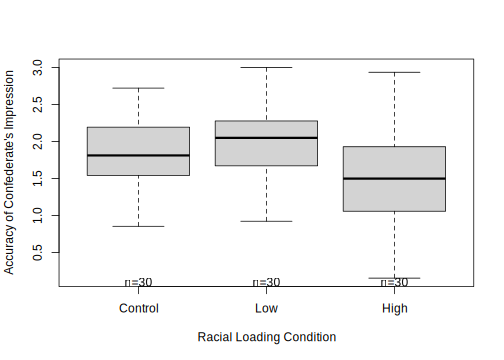
\includegraphics{ReCenterPsychStats_files/figure-latex/boxplot-1.pdf}

From both the boxplot and the linegraph with error bars, we can see that participants in the low racial loading condition have the highest accuracy ratings. This is followed by the control and then high racial loading conditions. Are these differences statistically significant? This is why we need the one-way ANOVA.

\hypertarget{understanding-anova-with-hand-calculations}{%
\section{\texorpdfstring{Understanding ANOVA with \emph{Hand Calculations}}{Understanding ANOVA with Hand Calculations}}\label{understanding-anova-with-hand-calculations}}

ANOVA was developed by Sir Ronald Fisher in the early 20th century. The name is a bit of a misnomer -- rather than analyzing \emph{variances}, we are investigating differences in \emph{means} (but the formula does take variances into consideration\ldots stay tuned).

ANOVA falls squarely within the tradition of \textbf{null hypothesis significance testing} (NHST). As such, a formal, traditional, ANOVA begins with statements of the null and alternate hypotheses. \emph{Note. Tran and Lee \citeyearpar{tran_you_2014} do not list such.}

In our example, we would hypothesize that the population means (i.e., Asian or Asian American individuals in the U.S.) are equal:

\[H_{O}:  \mu _{1} = \mu _{2} = \mu _{3}\]

There are an number of ways that the \(H_{O}\) could be false. Here are a few:

\[H_{a1}:  \mu _{1} \neq \mu _{2} \neq \mu _{3}\]
\[H_{a2}:  \mu _{1} =  \mu _{2} > \mu _{3}\]

\[H_{a3}:  \mu _{1} >  \mu _{2} > \mu _{3}\]
The bottom line is that if we have a statistically significant omnibus ANOVA (i.e., the test of the overall significance of the model) and the \(H_{O}\) is false, somewhere between the three levels of the grouping factor, the means are statistically significantly different from each other.

In evaluating the differences between means, one-way ANOVA compares:

\begin{itemize}
\tightlist
\item
  systematic variance to unsystematic variance
\item
  explained to unexplained variation
\item
  experimental effect to the individual differences
\item
  model variance to residual variance
\item
  between group variance to within group variance
\end{itemize}

The ratio of these variances is the \textbf{F-ratio}.

Navarro \citeyearpar{navarro_book_2020} offers a set of useful figures to compare between- and within-group variation.

\begin{figure}
\centering
\includegraphics{ReCenterPsychStats_files/figure-latex/unnamed-chunk-30-1.pdf}
\caption{\label{fig:unnamed-chunk-30}Graphical illustration of ``between groups'' variation}
\end{figure}

\begin{figure}
\centering
\includegraphics{ReCenterPsychStats_files/figure-latex/unnamed-chunk-31-1.pdf}
\caption{\label{fig:unnamed-chunk-31}Graphical illustration of ``within groups'' variation}
\end{figure}

Perhaps an oversimplification, but to the degree that between-group variance (i.e,. model variance) is greater than within-group variance (i.e., residual variance) there may be support to suggest that there are statistically significant differences between groups.

Let's examine how variance is partitioned by hand-calculating sums of squares total, model, and residual.

\hypertarget{sums-of-squares-total}{%
\subsection{Sums of Squares Total}\label{sums-of-squares-total}}

Sums of squares total represents the total amount of variance within our data. Examining the formula(s; there are several ways to consider it) can help us gain a conceptual understanding of this.

In this first version of the formula we can see that the grand (or overall) mean is subtracted from each individual score, squared, and then summed. This makes sense: \emph{sums of squares, total}.

\[SS_{T}= \sum (x_{i}-\bar{x}_{grand})^{2}\]
In the next version of the formula we see that the sums of square total is the addition of the sums of squares model and residual.

\[SS_{T}= SS_{M} + SS_{R}\]

``Between'' and ``within'' are another way to understand ``model'' and ``residual.'' This is reflected in the next formula.

\[SS_{T}= SS_{B} + SS_{W}\]
Finally, think of the sums of squares total as the grand variance multiplied by the overall degrees of freedom (\emph{N} - 1).

\[SS_{T}= s_{grand}^{2}(n-1)\]
Let's take a moment to \emph{hand-calculate} \(SS_{T}\). Not to worry! We'll get R to do the math for us. This is just a conceptual tour of sums of squares total.

Our grand (i.e., overall) mean is

\begin{Shaded}
\begin{Highlighting}[]
\FunctionTok{mean}\NormalTok{(accSIM30}\SpecialCharTok{$}\NormalTok{Accurate)}
\end{Highlighting}
\end{Shaded}

\begin{verbatim}
[1] 1.799009
\end{verbatim}

Subtracting the grand mean from each Accurate score yields a mean difference.

\begin{Shaded}
\begin{Highlighting}[]
\FunctionTok{library}\NormalTok{(tidyverse)}

\NormalTok{accSIM30 }\OtherTok{\textless{}{-}}\NormalTok{ accSIM30 }\SpecialCharTok{\%\textgreater{}\%} 
  \FunctionTok{mutate}\NormalTok{(}\AttributeTok{m\_dev =}\NormalTok{ Accurate}\SpecialCharTok{{-}}\FunctionTok{mean}\NormalTok{(Accurate))}
\end{Highlighting}
\end{Shaded}

Pop quiz: What's the sum of our new \emph{m\_dev} variable? Let's check.

\begin{Shaded}
\begin{Highlighting}[]
\FunctionTok{mean}\NormalTok{(accSIM30}\SpecialCharTok{$}\NormalTok{m\_dev)}
\end{Highlighting}
\end{Shaded}

\begin{verbatim}
[1] -0.00000000000000005421372
\end{verbatim}

R uses \textbf{scientific e notation}. The proper value is one where the base number (before the ``e'') is multiplied by 10, raised to the power shown: \(5.421372 * 10^{17}\) Another way to think of it is to move the decimal 17 places to the left. In any case, this number is essentially zero.

Back to the point of sums of squares total, the sum of deviations around the grand mean will always be zero. To make them useful, we must square them:

\begin{Shaded}
\begin{Highlighting}[]
\NormalTok{accSIM30 }\OtherTok{\textless{}{-}}\NormalTok{ accSIM30 }\SpecialCharTok{\%\textgreater{}\%} 
  \FunctionTok{mutate}\NormalTok{(}\AttributeTok{m\_devSQ =}\NormalTok{ m\_dev}\SpecialCharTok{\^{}}\DecValTok{2}\NormalTok{)}
\end{Highlighting}
\end{Shaded}

If we sum the squared mean deviations we will obtain the total variance (sums of squares total):

\begin{Shaded}
\begin{Highlighting}[]
\FunctionTok{sum}\NormalTok{(accSIM30}\SpecialCharTok{$}\NormalTok{m\_devSQ)}
\end{Highlighting}
\end{Shaded}

\begin{verbatim}
[1] 38.34623
\end{verbatim}

This value, the sum of squared deviations around the grand mean, is our \(SS_T\); the associated \emph{degrees of freedom} is \(N - 1\); in our case this is 90-1 = 89.

In one-way ANOVA, we divide \(SS_T\) into \textbf{model/between sums of squares} and \textbf{residual/within sums of squares}.

The \emph{model} generally represents the notion that the means are different than each other. We want the variation between our means to be greater than the variation within each of the groups from which our means are calculated.

\hypertarget{sums-of-squares-for-the-model-or-between}{%
\subsection{Sums of Squares for the Model (or Between)}\label{sums-of-squares-for-the-model-or-between}}

We just determined that the total amount of variation within the data is 38.35 units. From this we can estimate how much of this variation our model can explain. \(SS_M\) tells us how much of the total variation can be explained by the fact that different data points come from different groups.

We see this reflected in the formula below, where

\begin{itemize}
\tightlist
\item
  the grand mean is subtracted from each group mean
\item
  this value is squared and multiplied by the number of cases in each group
\item
  these values are summed
\end{itemize}

\[SS_{M}= \sum n_{k}(\bar{x}_{k}-\bar{x}_{grand})^{2}\]

To calculate this, we start with the grand mean.

\begin{Shaded}
\begin{Highlighting}[]
\FunctionTok{mean}\NormalTok{(accSIM30}\SpecialCharTok{$}\NormalTok{Accurate)}
\end{Highlighting}
\end{Shaded}

\begin{verbatim}
[1] 1.799009
\end{verbatim}

We also estimate the group means.

\begin{Shaded}
\begin{Highlighting}[]
\FunctionTok{aggregate}\NormalTok{ (Accurate }\SpecialCharTok{\textasciitilde{}}\NormalTok{ COND, accSIM30, mean)}
\end{Highlighting}
\end{Shaded}

\begin{verbatim}
     COND Accurate
1 Control 1.876882
2     Low 2.046506
3    High 1.473640
\end{verbatim}

This formula occurs in three chunks, representing the control, low, and high racial loading conditions. In each of the chunks we have the \(n\), group mean, and grand mean.

\begin{Shaded}
\begin{Highlighting}[]
\DecValTok{30}\SpecialCharTok{*}\NormalTok{(}\FloatTok{1.876} \SpecialCharTok{{-}} \FloatTok{1.799}\NormalTok{)}\SpecialCharTok{\^{}}\DecValTok{2} \SpecialCharTok{+} \DecValTok{30}\SpecialCharTok{*}\NormalTok{(}\FloatTok{2.046} \SpecialCharTok{{-}} \FloatTok{1.799}\NormalTok{)}\SpecialCharTok{\^{}}\DecValTok{2} \SpecialCharTok{+} \DecValTok{30}\SpecialCharTok{*}\NormalTok{(}\FloatTok{1.474} \SpecialCharTok{{-}} \FloatTok{1.799}\NormalTok{)}\SpecialCharTok{\^{}}\DecValTok{2}
\end{Highlighting}
\end{Shaded}

\begin{verbatim}
[1] 5.17689
\end{verbatim}

This value, \(SS_M\) is the value accounted for by the model -- the proportion of variance accounted for by the grouping variable/factor, COND. Degrees of freedom for \(SS_M\) is always one less than the number of elements (e.g., groups) used in its calculation (\(k-1\)). Because we have three groups, our degrees of freedom for the model is 2.

\hypertarget{sums-of-squares-residual-or-within}{%
\subsection{Sums of Squares Residual (or within)}\label{sums-of-squares-residual-or-within}}

To recap, we know there are 38.35 units of variation to be explained in our data. Our model explains 5.18 of these units. Sums of squares residual tells us how much of the variation cannot be explained by the model. This value is influenced by extraneous factors; some will refer to it as ``noise.''

Looking at the formula can assist us in with a conceptual formula. In \(SS_R\) we subtract the group mean from each individual member of the group and then square it.

\[SS_{R}= \sum(x_{ik}-\bar{x}_{k})^{^{2}}\]
Here's another approach to calculating\(SS_R\). In this one the variance for each group is multiplied by its respective degrees of freedom, then summed.

\[SS_{R}= s_{group1}^{2}(n-1) + s_{group2}^{2}(n-1) + s_{group3}^{2}(n-1))\]
Again, the formula is in three chunks -- but this time the calculations are \emph{within-group}. We need the variance (the standard deviation squared) for the calculation.

\begin{Shaded}
\begin{Highlighting}[]
\FunctionTok{aggregate}\NormalTok{ (Accurate }\SpecialCharTok{\textasciitilde{}}\NormalTok{ COND, accSIM30, sd)}
\end{Highlighting}
\end{Shaded}

\begin{verbatim}
     COND  Accurate
1 Control 0.4791969
2     Low 0.5725299
3    High 0.7653157
\end{verbatim}

A quick tangent -- this calculation demonstrates the relationship between standard deviation and variance. Variance is the standard deviation, squared.

\begin{Shaded}
\begin{Highlighting}[]
\CommentTok{\#just showing you that the variance (next) is the standard deviation, squared}
\NormalTok{.}\DecValTok{4791969}\SpecialCharTok{\^{}}\DecValTok{2}
\end{Highlighting}
\end{Shaded}

\begin{verbatim}
[1] 0.2296297
\end{verbatim}

\begin{Shaded}
\begin{Highlighting}[]
\FunctionTok{aggregate}\NormalTok{ (Accurate }\SpecialCharTok{\textasciitilde{}}\NormalTok{ COND, accSIM30, var)}
\end{Highlighting}
\end{Shaded}

\begin{verbatim}
     COND  Accurate
1 Control 0.2296297
2     Low 0.3277905
3    High 0.5857082
\end{verbatim}

We will use the second formula to calculate \(SS_R\). For each of the groups, we multiply the variance by the respective degrees of freedom for the group (\emph{n} - 1).

\begin{Shaded}
\begin{Highlighting}[]
\NormalTok{.}\DecValTok{2296}\SpecialCharTok{*}\NormalTok{(}\DecValTok{30{-}1}\NormalTok{) }\SpecialCharTok{+}\NormalTok{ .}\DecValTok{3278}\SpecialCharTok{*}\NormalTok{(}\DecValTok{30{-}1}\NormalTok{) }\SpecialCharTok{+}\NormalTok{ .}\DecValTok{5857}\SpecialCharTok{*}\NormalTok{(}\DecValTok{30{-}1}\NormalTok{)}
\end{Highlighting}
\end{Shaded}

\begin{verbatim}
[1] 33.1499
\end{verbatim}

The value for our \(SS_R\) is 33.15. Degrees of freedom for the residual is \(df_T - df_M\).

\begin{itemize}
\tightlist
\item
  \(df_T\) was \(N-1\): 90 - 1 = 89
\item
  \(df_M\) was \(k - 1\): 3 - 1 = 2
\item
  Therefore, \(df_R\): is 89 - 2 = 87
\end{itemize}

\hypertarget{relationship-between-ss_t-ss_m-and-ss_r.}{%
\subsection{\texorpdfstring{Relationship between \(SS_T\), \(SS_M\), and \(SS_R\).}{Relationship between SS\_T, SS\_M, and SS\_R.}}\label{relationship-between-ss_t-ss_m-and-ss_r.}}

In case it's not clear:

\(SS_T = SS_M + SS_R\)

\begin{Shaded}
\begin{Highlighting}[]
\FloatTok{33.15} \SpecialCharTok{+} \FloatTok{5.18}
\end{Highlighting}
\end{Shaded}

\begin{verbatim}
[1] 38.33
\end{verbatim}

\emph{The difference (38.35 vs.~38.33) is likely due to rounding error. Earlier estimates had multiple decimal points.}

\hypertarget{mean-squares-model-residual}{%
\subsection{Mean Squares Model \& Residual}\label{mean-squares-model-residual}}

Our estimates of variation were \emph{sums of squares} and are influenced by the number of scores that were summed. We can correct this bias by calculating their average -- the \emph{mean squares} or \(MS\). We will use these in the calculation of the \(F\) statistic -- the statistic that tests if there are significant differences between groups.

Like the constellation of sums of squares, we calculate mean squares for the model (\(MS_M\)) and residual(\(MS_R\)). Each formula simply divides the corresponding sums of squares by their respective degrees of freedom.

\[MS_M = \frac{SS_{M}}{df{_{M}}}\]

Regarding the calculation of our model mean squares:

\begin{itemize}
\tightlist
\item
  \(SS_M\) was 5.17689
\item
  \(df_M\) was 2
\item
  Therefore, \(MS_M=\)is:
\end{itemize}

\begin{Shaded}
\begin{Highlighting}[]
\CommentTok{\# mean squares for the model}
\FloatTok{5.17689}\SpecialCharTok{/}\DecValTok{2}
\end{Highlighting}
\end{Shaded}

\begin{verbatim}
[1] 2.588445
\end{verbatim}

\[MS_R = \frac{SS_{R}}{df{_{R}}}\]
Regarding the calculation of our model residual squares:

\begin{itemize}
\tightlist
\item
  \(SS_R\) was 33.1499
\item
  \(df_R\) was 87
\item
  Therefore, \(MS_R\) is:
\end{itemize}

\begin{Shaded}
\begin{Highlighting}[]
\CommentTok{\# mean squares for the residual}
\FloatTok{33.1499} \SpecialCharTok{/} \DecValTok{87}
\end{Highlighting}
\end{Shaded}

\begin{verbatim}
[1] 0.3810333
\end{verbatim}

\hypertarget{calculating-the-f-statistic}{%
\subsection{\texorpdfstring{Calculating the \emph{F}-Statistic}{Calculating the F-Statistic}}\label{calculating-the-f-statistic}}

The \emph{F}-statistic (or \emph{F}-ratio) is the assesses the ratio (as its name implies) of variation explained by the model to unsystematic factors (i.e., the residual). Earlier we used ``between'' and ``within'' language. Especially when we think of our example -- where the model is composed of three groups, we can think of the \emph{F} statistic as assessing the ratio of variation explained by between-subjects differences to within-subjects differences. Navarro's \citep{navarro_chapter_2020} figures (earlier in the chapter) illustrate this well.

\[F = \frac{MS_{M}}{MS_{R}}\]
Regarding the calculation of our \emph{F}-ratio:

\begin{itemize}
\tightlist
\item
  \(MS_M\) was 2.588445
\item
  \(MS_R\) was 0.3810333
\item
  Therefore, \(F\) is:
\end{itemize}

\begin{Shaded}
\begin{Highlighting}[]
\FloatTok{2.588445} \SpecialCharTok{/} \FloatTok{0.3810333}
\end{Highlighting}
\end{Shaded}

\begin{verbatim}
[1] 6.793225
\end{verbatim}

\hypertarget{source-table-games}{%
\subsection{Source Table Games}\label{source-table-games}}

These last few calculations are actually less complicated than this presentation makes them seem. To better understand the relation between sums of squares, degrees of freedom, and mean squares, let's play a couple of rounds of \emph{Source Table Games}!

Rules of the game:

\begin{itemize}
\tightlist
\item
  In each case, mean squares are determined by dividing the sums of squares by its respective degrees of freedom.
\item
  The F statistic is determined by dividing \(MS_M\) by \(MS_R\)
\end{itemize}

Knowing only two of the values, challenge yourself to complete the rest of the table. Before looking at the answers (below), try to the fill in the blanks based in the table based on what we have learned so far.

\begin{longtable}[]{@{}lrrr@{}}
\toprule
Game & Total (df, \emph{N} - 1) & Model (df, \emph{k} -1) & Residual (df, \(df_T - df_M\)) \\
\midrule
\endhead
SS & 38.346(89) & 5.17689(2) & \_\_\_\_\_\_ \\
MS & NA & \_\_\_\_\_\_ & \_\_\_\_\_\_ \\
\bottomrule
\end{longtable}

\(F = MS_{M}/MS_{R}\) = \_\_\_\_\_\_

\textbf{DON'T PEEK! TRY TO DO THE CALCULATIONS IN THE ``SOURCE TABLE GAMES'' EXERCISE BEFORE LOOKING AT THESE ANSWERS}

\begin{longtable}[]{@{}lrrr@{}}
\toprule
Answers & Total (df, \emph{N} - 1) & Model (df, \emph{k} -1) & Residual (df, \(df_T - df_M\)) \\
\midrule
\endhead
SS & 38.346(89) & 5.17689(2) & 33.1499(87) \\
MS & NA & 2.5885 & 0.38103 \\
\bottomrule
\end{longtable}

\(F = MS_{M}/MS_{R}\) = 6.973

To determine whether or not it is statistically significant, we can check a \href{https://www.statology.org/how-to-read-the-f-distribution-table/}{table of critical values} \citep{zach_how_2019} for the \emph{F} test.

Our example has 2 (numerator) and 87 (denominator) degrees of freedom. Rolling down to the table where \(\alpha = .05\), we can see that any \(F\) value \textgreater{} 3.11 (a value somewhere between 3.07 and 3.15) will be statistically significant. Our \(F\) = 6.79, so we have clearly exceeded the threshold. This is our \emph{omnibus F test}. Significance at this level lets us know that there is at least 1 statistically significant difference between our control, low, and high racially loaded conditions. While it is important to follow-up to see where these significant differences lie, we will not do these by hand. Rather, let's rework the problem in R.

\hypertarget{working-the-one-way-anova-in-r}{%
\section{Working the One-Way ANOVA in R}\label{working-the-one-way-anova-in-r}}

Let's rework the problem in R. We start at the top of the flowchart, evaluating the statistical assumptions.

\begin{figure}
\centering
\includegraphics{images/OnewayWrkFlw_Asmptns.jpg}
\caption{An image of the workflow for one-way ANOVA, showing that we are at the beginning: evaluating the potential violation of the assumptions.}
\end{figure}

\hypertarget{evaluating-the-statistical-assumptions}{%
\subsection{Evaluating the Statistical Assumptions}\label{evaluating-the-statistical-assumptions}}

All statistical tests have some assumptions about the data. The one-way ANOVA has four assumptions:

\begin{itemize}
\tightlist
\item
  The dependent variable is normally distributed for each of the populations as defined by the different levels of the factor. We will examine this by

  \begin{itemize}
  \tightlist
  \item
    evaluating skew and kurtosis
  \item
    visually inspecting the distribution
  \item
    conduct a Shapiro Wilks test
  \item
    examine a QQ plot
  \end{itemize}
\item
  The variances of the dependent variable are the same for all populations. This is often termed the \emph{homogeneity of variance} assumption. We will examine this with

  \begin{itemize}
  \tightlist
  \item
    Levene's Test
  \end{itemize}
\item
  The cases represent \emph{random} samples from the populations and scores on the test variable are independent of each other. That is, comparing related cases (e.g., parent/child, manager/employee, time1/time2) must be completed by another statistic such as repeated measures ANOVA or dyadic data analysis.

  \begin{itemize}
  \tightlist
  \item
    \emph{Independence} in observations is a research design issue. ANOVA not robust to violating this assumption. When observations are correlated/dependent there is a dramatic increase in Type I error.
  \end{itemize}
\item
  The dependent variable is measured on an interval scale.

  \begin{itemize}
  \tightlist
  \item
    This is also a research design issue. If the dependent variable is categorical, another statistic (such as logistic regression) should be chosen.
  \end{itemize}
\end{itemize}

\hypertarget{is-the-dependent-variable-normally-distributed-across-levels-of-the-factor}{%
\subsubsection{Is the dependent variable normally distributed across levels of the factor?}\label{is-the-dependent-variable-normally-distributed-across-levels-of-the-factor}}

From the \emph{psych} package, the \emph{describe()} function can be used to provide descriptives of continuously scaled variables (i.e., variables measured on the interval or ratio scale). In this simple example, we can specify the specific continuous, DV.

\begin{Shaded}
\begin{Highlighting}[]
\FunctionTok{library}\NormalTok{(psych)}
\CommentTok{\#we name the function}
\CommentTok{\#in parentheses we list the object that is the dataframe}
\CommentTok{\#the $ sign precedes the specific variable for which we want the information}
\FunctionTok{describe}\NormalTok{(accSIM30}\SpecialCharTok{$}\NormalTok{Accurate)}
\end{Highlighting}
\end{Shaded}

\begin{verbatim}
   vars  n mean   sd median trimmed  mad  min max range  skew kurtosis   se
X1    1 90  1.8 0.66    1.8    1.83 0.56 0.15   3  2.85 -0.33    -0.07 0.07
\end{verbatim}

If we want descriptives for each level of the grouping variable (factor), we can use the \emph{describeBy()} function of the \emph{psych} package. The order of entry within the script is the DV followed by the grouping variable (IV).

\begin{Shaded}
\begin{Highlighting}[]
\CommentTok{\#It is unnecessary to create an object, but an object allows you to do cool stuff, like write it to a .csv file and use that as a basis for APA style tables}
\CommentTok{\#In this script we can think "Accurate by COND" meaning that the descriptives for accuracy will be grouped by COND which is a categorical variable}
\CommentTok{\#mat = TRUE means we will get the output in matrix (table) form}
\CommentTok{\#digits = 3 means output will be rounded to 3 decimal places}
\CommentTok{\#data = accSIM30 is a different (I think easier) way to identify the object that holds the dataframe}
\NormalTok{des.mat }\OtherTok{\textless{}{-}} \FunctionTok{describeBy}\NormalTok{ (Accurate }\SpecialCharTok{\textasciitilde{}}\NormalTok{ COND, }\AttributeTok{mat=}\ConstantTok{TRUE}\NormalTok{, }\AttributeTok{digits=}\DecValTok{3}\NormalTok{, }\AttributeTok{data=}\NormalTok{accSIM30) }

\CommentTok{\#describeBy(accSIM30$Accurate, accSIM30$COND, mat=TRUE)}

\NormalTok{des.mat }\CommentTok{\#let\textquotesingle{}s you see the matrix object}
\end{Highlighting}
\end{Shaded}

\begin{verbatim}
    item  group1 vars  n  mean    sd median trimmed   mad   min   max range
X11    1 Control    1 30 1.877 0.479  1.811   1.872 0.460 0.854 2.721 1.867
X12    2     Low    1 30 2.047 0.573  2.049   2.053 0.534 0.922 3.000 2.078
X13    3    High    1 30 1.474 0.765  1.498   1.469 0.646 0.153 2.935 2.782
      skew kurtosis    se
X11  0.134   -0.756 0.087
X12  0.017   -0.872 0.105
X13 -0.034   -0.789 0.140
\end{verbatim}

\begin{Shaded}
\begin{Highlighting}[]
\FunctionTok{write.csv}\NormalTok{ (des.mat, }\AttributeTok{file=}\StringTok{"Table1.csv"}\NormalTok{) }\CommentTok{\#optional to write it to a .csv file}
\end{Highlighting}
\end{Shaded}

Skew and kurtosis speaks to normal distributions. The skew and kurtosis indices in the \emph{psych} package are reported as \emph{z} scores. Regarding skew, values greater than 3.0 are generally considered ``severely skewed.'' Regarding kurtosis, ``severely kurtotic'' is argued to be anywhere greater 8 to 20 \citep{kline_principles_2016}.

The \emph{Shapiro-Wilks} test evaluates the hypothesis that the distribution of the data as a whole deviates from a comparable normal distribution. If the test is non-significant (\emph{p} \textgreater.05) it tells us that the distribution of the sample is not significantly different from a normal distribution. If, however, the test is significant (\emph{p} \textless{} .05) then the distribution in question is significantly different from a normal distribution.

\begin{Shaded}
\begin{Highlighting}[]
\FunctionTok{shapiro.test}\NormalTok{(accSIM30}\SpecialCharTok{$}\NormalTok{Accurate)}
\end{Highlighting}
\end{Shaded}

\begin{verbatim}
    Shapiro-Wilk normality test

data:  accSIM30$Accurate
W = 0.97413, p-value = 0.06931
\end{verbatim}

The \(p\) value (\(p\) = 0.069) is just barely above .05. This tells us that the Accurate variable does not deviate from a statistically significant distribution.

There are limitations to the Shapiro-Wilks test. As the dataset being evaluated gets larger, the Shapiro-Wilks test becomes more sensitive to small deviations; this leads to a greater probability of rejecting the null hypothesis (null hypothesis being the values come from a normal distribution). Green and Salkind \citeyearpar{green_using_2014} advised that ANOVA is relatively robust to violations of normality if there are at least 15 cases per cell and the design is reasonably balanced (i.e., equal cell sizes).

So, is our dependent variable normally distributed at each of the levels of the factor? In statistics we generally provide cautious and tentative answers. My interpretation is that there is not evidence to suggest that we have violated this assumption.

\hypertarget{are-the-variances-of-the-dependent-variable-similar-across-the-levels-of-the-grouping-factor}{%
\subsubsection{Are the variances of the dependent variable similar across the levels of the grouping factor?}\label{are-the-variances-of-the-dependent-variable-similar-across-the-levels-of-the-grouping-factor}}

The Levene's test evaluates the ANOVA assumption that variances of the dependent variable for each level of the independent variable are similarly distributed. We want this to be non-significant (\(p\) \textgreater{} .05). If violated, we need to use an ANOVA test that is ``robust to the violation of the homogeneity of variance'' (e.g., Welch's oneway).

In R, Levene's test is found in the \emph{car} package.

\begin{Shaded}
\begin{Highlighting}[]
\FunctionTok{library}\NormalTok{(car)}
\end{Highlighting}
\end{Shaded}

\begin{verbatim}
Loading required package: carData
\end{verbatim}

\begin{verbatim}
Attaching package: 'car'
\end{verbatim}

\begin{verbatim}
The following object is masked from 'package:dplyr':

    recode
\end{verbatim}

\begin{verbatim}
The following object is masked from 'package:purrr':

    some
\end{verbatim}

\begin{verbatim}
The following object is masked from 'package:psych':

    logit
\end{verbatim}

\begin{Shaded}
\begin{Highlighting}[]
\CommentTok{\#Our set up is similar:  Accurate by condition, followed by the object that holds the dataframe, followed by the instruction to center the analysis around the mean}
\FunctionTok{leveneTest}\NormalTok{ (Accurate }\SpecialCharTok{\textasciitilde{}}\NormalTok{ COND, accSIM30, }\AttributeTok{center=}\NormalTok{mean)}
\end{Highlighting}
\end{Shaded}

\begin{verbatim}
Levene's Test for Homogeneity of Variance (center = mean)
      Df F value Pr(>F)
group  2   2.274  0.109
      87               
\end{verbatim}

We write the result of the Levene's as \(F\)(2,87) = 2.274, \(p\) = 0.109 Because \(p\) \textgreater{} .05, we know that the result is nonsignficant -- that the variances of the three groups are not statistically significantly different than each other.

IF the results had been statistically significantly different, we would have needed to use a Welch's \(F\) or robust version of ANOVA.

\hypertarget{summarizing-results-from-the-analysis-of-assumptions}{%
\subsubsection{Summarizing results from the analysis of assumptions}\label{summarizing-results-from-the-analysis-of-assumptions}}

It is common for an APA style results section to begin with a review of the evaluation of the statistical assumptions. As we have just finished these analyses, I will document what we have learned so far:

A one-way analysis of variance was conducted to evaluate the relationship between degree of racial loading of an exceptionalizing microaggression and the perceived accuracy of a research confederate's impression of the Asian or Asian American participant. The independent variable, COND, included three levels: control/none, low, and high levels of racial loading. Results of Levene's homogeneity of variance test indicated no violation of the homogeneity of variance assumption (\(F\){[}(2,87{]} = 2.274, \(p\) = 0.109 ). Similarly, results of the Shapiro Wilk's test indicated no violation of the normality assumption \emph{W} = 0.97413, \emph{p} = 0.069.

Now we can move onto computing the omnibus ANOVA. \emph{Omnibus} is the term applied to the first \emph{F} test that evaluates if all groups have the same mean \citep{chen_relationship_2018}. If this test is not significance there is no evidence in the data to reject the null; that is, there is no evidence to suggest that group means are different. If it is significant -- and there are 3 or more groups -- follow-up testing will be needed to determine where the differences lie.

\hypertarget{computing-the-omnibus-anova}{%
\subsection{Computing the Omnibus ANOVA}\label{computing-the-omnibus-anova}}

Having met all the assumptions, we are now ready to calculate the omnibus \(F\) test.

\begin{figure}
\centering
\includegraphics{images/OnewayWrkFlw_omnibus.jpg}
\caption{An image of the workflow for one-way ANOVA, showing that we are at the stage of computing the omnibus ANOVA.}
\end{figure}

ANOVA is a special case of the general linear model (regression is a ``not so special case'' of the general linear model), therefore we use the linear model function, \emph{aov()} to run the analysis.

In the code below, we predict Accuracy from COND (3 levels: control, low, high).

By assigning the results of the \emph{aov()} function to an object (accBYcond) we can then use that object (think \emph{model}) in other functions to get details about our analysis.

\begin{Shaded}
\begin{Highlighting}[]
\CommentTok{\#the script looks familiar, "Accurate by Condition"}
\NormalTok{accBYcond }\OtherTok{\textless{}{-}} \FunctionTok{aov}\NormalTok{(Accurate }\SpecialCharTok{\textasciitilde{}}\NormalTok{ COND, }\AttributeTok{data =}\NormalTok{ accSIM30) }\CommentTok{\#DV \textasciitilde{} IV  I say, "DV by IV"}
\FunctionTok{summary}\NormalTok{ (accBYcond) }\CommentTok{\#ANOVA output}
\end{Highlighting}
\end{Shaded}

\begin{verbatim}
            Df Sum Sq Mean Sq F value  Pr(>F)   
COND         2   5.20   2.598   6.817 0.00178 **
Residuals   87  33.15   0.381                   
---
Signif. codes:  0 '***' 0.001 '**' 0.01 '*' 0.05 '.' 0.1 ' ' 1
\end{verbatim}

Inserting the \emph{aov()} object (accBYcond) into the summary command produces the ANOVA Source Table that we manually created above.

The values we see map onto those we calculated by hand. Our \(SS_M\) (5.20) plus \(SS_R\) (33.15) add to the \(SS_T\) (38.35) we calculated by hand.

Dividing the two sums of squares by their respective degrees of freedom produces the sums of means squared.

Then, dividing the \(MS_M\) (COND) by \(MS_R\) (2.598/-.381) provides the \emph{F} value. By using a table of \emph{F} critical values, we already knew that our \emph{F} value exceeded the value in the table of critical values. Here we see that \emph{p} = 0.00178.

The ``\emph{F} string'' for an APA style results section should be written like this: \emph{F} (2, 87) = 6.817, \emph{p} = 0.002.

The object we created with the \emph{aov()} function is capable of producing much information. Applying the \emph{names()} function to the object can give us a list of values within it.

\begin{Shaded}
\begin{Highlighting}[]
\FunctionTok{names}\NormalTok{(accBYcond)}
\end{Highlighting}
\end{Shaded}

\begin{verbatim}
 [1] "coefficients"  "residuals"     "effects"       "rank"         
 [5] "fitted.values" "assign"        "qr"            "df.residual"  
 [9] "contrasts"     "xlevels"       "call"          "terms"        
[13] "model"        
\end{verbatim}

\emph{summary()} is one of the most commonly used function applied to \emph{aov()} objects, but it's not the only one.
Let's try some other options.

\begin{Shaded}
\begin{Highlighting}[]
\FunctionTok{model.tables}\NormalTok{ (accBYcond, }\StringTok{"means"}\NormalTok{)}
\end{Highlighting}
\end{Shaded}

\begin{verbatim}
Tables of means
Grand mean
         
1.799009 

 COND 
COND
Control     Low    High 
 1.8769  2.0465  1.4736 
\end{verbatim}

Let's graph some of the data.

\begin{Shaded}
\begin{Highlighting}[]
\FunctionTok{plot}\NormalTok{(accBYcond) }
\end{Highlighting}
\end{Shaded}

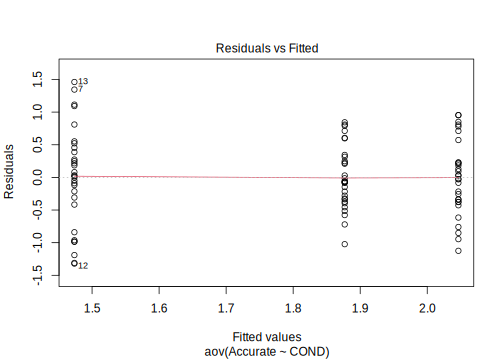
\includegraphics{ReCenterPsychStats_files/figure-latex/plot function-1.pdf} 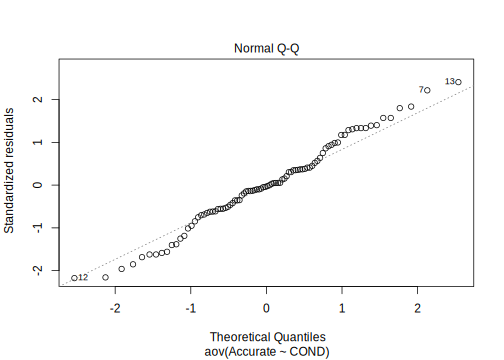
\includegraphics{ReCenterPsychStats_files/figure-latex/plot function-2.pdf} 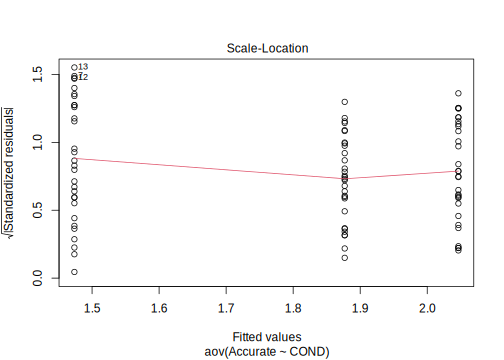
\includegraphics{ReCenterPsychStats_files/figure-latex/plot function-3.pdf} 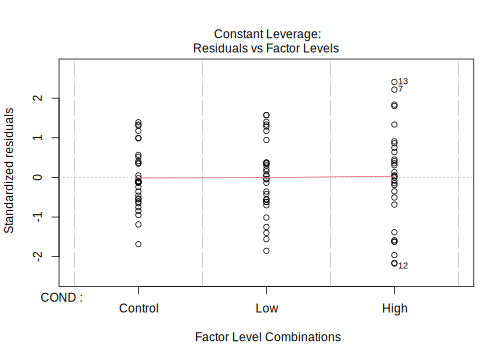
\includegraphics{ReCenterPsychStats_files/figure-latex/plot function-4.pdf}

The \emph{aov()} command has a quickplot feature. The first of the four plots fits the residuals. We already know from Levene's that we did not violate the homogeneity of variance test. With its straight line, this plot shows an equal spread across the three groups.

When the dots of the Q-Q plot map onto the diagonal, we have some indication of normality of the residuals (we want residuals to be normally distributed).

\hypertarget{effect-size-for-the-one-way-anova}{%
\subsubsection{Effect size for the one-way ANOVA}\label{effect-size-for-the-one-way-anova}}

\textbf{Eta squared} is one of the most commonly used measures of effect. It refers to the proportion of variability in the dependent variable/outcome that can be explained in terms of the independent variable/predictor. Traditional interpretive values are similar to the Pearson's \emph{r}:

0 = no relationship
.02 = small
.13 = medium
.26 = large
1 = a perfect (one-to-one) correspondence

A useful summary of effect sizes, guide to interpreting their magnitudes, and common usage can be found \href{https://imaging.mrc-cbu.cam.ac.uk/statswiki/FAQ/effectSize}{here} \citep{watson_rules_2020}.

The formula for \(\eta^2\) is straightforward. If we think back to our hand-calculations of all the sums of squares, we can clearly see that this is the proportion of variance that is accounted for by the model.

\[\eta ^{2}=\frac{SS_{M}}{SS_{T}}\]
Hand calculation, then, is straightforward.:

\begin{Shaded}
\begin{Highlighting}[]
\FloatTok{5.20} \SpecialCharTok{/}\NormalTok{ (}\FloatTok{5.20} \SpecialCharTok{+} \FloatTok{33.15}\NormalTok{)}
\end{Highlighting}
\end{Shaded}

\begin{verbatim}
[1] 0.1355932
\end{verbatim}

The \emph{lsr} package includes an eta-squared calculator. To use it, we simply insert the model/object we created with the \emph{aov()} function to \emph{lsr}'s \emph{etaSquared()} function.

\begin{Shaded}
\begin{Highlighting}[]
\FunctionTok{library}\NormalTok{(lsr)}
\FunctionTok{etaSquared}\NormalTok{(accBYcond)}
\end{Highlighting}
\end{Shaded}

\begin{verbatim}
        eta.sq eta.sq.part
COND 0.1354894   0.1354894
\end{verbatim}

Notice that there are two effect sizes. We described eta-squared. Partial eta-squared is the effect size reported in SPSS. There's a long history of debate about which to use. In certain circumstances (especially in more complicated analyses), partial-eta squared can be a bit more generous (i.e., larger than \(\eta^2\)). Thus, many prefer the reporting of \(\eta^2\).

In our case, we see no difference between the two values. Differences begin to appear in datasets that are more complicated, such as when sample sizes across the levels of a factor differ.

\hypertarget{summarizing-results-from-the-omnibus-anova}{%
\subsubsection{Summarizing results from the omnibus ANOVA}\label{summarizing-results-from-the-omnibus-anova}}

Presenting the APA style results of the omnibus test is very straightforward:

Results indicated a significant effect of COND on accuracy perception \$ F(2, 87) = 6.817, p = 0.002, \eta\^{}2 = .14\$.

\hypertarget{follow-up-to-the-omnibus-f}{%
\subsection{\texorpdfstring{Follow-up to the Omnibus \emph{F}}{Follow-up to the Omnibus F}}\label{follow-up-to-the-omnibus-f}}

The \emph{F}-test associated with the one-way ANOVA is the \emph{omnibus} -- giving the result for the overall test. Looking at the workflow for the one-way ANOVA we see that if we had had we had a non-significant \(F\), we would have stopped our analysis.

However, if the omnibus \(F\) is significant, we know that there is at least one pair of cells where there is a statistically significant difference. We have several ways (each with its own strengths/limitations) to figure out where these differences lie.

We have several options for following up; a very common option is to conduct post-hoc, pairwise comparisons.

\begin{figure}
\centering
\includegraphics{images/OnewayWrkFlw_phoc.jpg}
\caption{An image of the workflow for one-way ANOVA, showing that we are at the stage of following a statistically significant omnibus F test and are now conducting posthoc comparisons.}
\end{figure}

\hypertarget{option-1-post-hoc-pairwise-comparisons}{%
\subsubsection{OPTION 1: Post-hoc, pairwise, comparisons}\label{option-1-post-hoc-pairwise-comparisons}}

Post-hoc, pairwise comparisons are:

\begin{itemize}
\tightlist
\item
  used for exploratory work when no firm hypotheses were articulated a priori,
\item
  used to compare the means of all combinations of pairs of an experimental condition,
\item
  less powerful than planned comparisons b/c strict criterion for significance must be used.
\end{itemize}

Helpful information about how to conduct post-hoc pairwise comparisons in R can be found at the \href{https://stats.idre.ucla.edu/r/faq/how-can-i-do-post-hoc-pairwise-comparisons-in-r/}{UCLA Institute for Digital Research and Education site} \citep{noauthor_how_nodate}.

\begin{Shaded}
\begin{Highlighting}[]
\FunctionTok{pairwise.t.test}\NormalTok{(accSIM30}\SpecialCharTok{$}\NormalTok{Accurate, accSIM30}\SpecialCharTok{$}\NormalTok{COND, }\AttributeTok{p.adj =} \StringTok{"none"}\NormalTok{)}
\end{Highlighting}
\end{Shaded}

\begin{verbatim}
    Pairwise comparisons using t tests with pooled SD 

data:  accSIM30$Accurate and accSIM30$COND 

     Control Low    
Low  0.29016 -      
High 0.01321 0.00054

P value adjustment method: none 
\end{verbatim}

\begin{Shaded}
\begin{Highlighting}[]
\CommentTok{\#can swap "bonf" or "holm" for p.adj}
\end{Highlighting}
\end{Shaded}

The output only provides the \(p\) values associated with the mean differences in each of the conditions. We see that \(p < .05\) when control is compared to low. An APA style reporting results of these typically involves referencing the means (often reported in a table of means and standard deviations) or mean differences (hand calculated) with their \emph{p} values.

\textbf{Should we be concerned about Type I error?"}

Recall that \emph{Type I error} is the concern about false positives -- that we would incorrectly reject a true null hypothesis (that we would say that there is a statistically significant difference when there is not one). This concern increases when we have a large number of pairwise comparisons.

Green and Salkind \citeyearpar{green_using_2014} review three options for managing Type I error.

\begin{itemize}
\tightlist
\item
  Traditional Bonferroni:

  \begin{itemize}
  \tightlist
  \item
    Adjusts the \emph{p} value upward by multiplying it (the raw \emph{p} values) by the number of comparisons being completed. This holds the \emph{total} Type I error rate across these tests to \(\alpha\) (usually .05). The traditional Bonferroni is simple and therefore attractive, but when \emph{p} values hover around .05, it can be too restrictive.
  \end{itemize}
\item
  Holms Sequential Bonferroni:

  \begin{itemize}
  \tightlist
  \item
    We'll describe this in more detail later. Briefly, it allows us to rank order the comparisons by their \emph{p} value (smallest to largest). We determine the significance of each \emph{p} value \emph{sequentially.}\\
  \end{itemize}
\item
  LSD method:

  \begin{itemize}
  \tightlist
  \item
    Permitted when there are only three pairwise comparisons among three groups, researchers can leave the \emph{p} values as they are. Since the Tran and Lee \citeyearpar{tran_you_2014} research vignette is one of those circumstances, I not make adjustments for Type I error. I would name claim the LSD and cite Green and Salkind {[}-green\_using\_2014{]} as justification for that decision.
  \end{itemize}
\end{itemize}

There is, though, an even more powerful approach\ldots{}

\hypertarget{option-2-planned-contrasts}{%
\subsubsection{OPTION 2: Planned contrasts}\label{option-2-planned-contrasts}}

Another option is to evaluate planned comparisons.

\includegraphics{images/OnewayWrkFlw_planned.jpg}
Planned comparisons are

\begin{itemize}
\tightlist
\item
  theory-driven comparisons constructed prior to data collection,
\item
  based on the idea of partitioning the variance created by the overall effect of group differences into gradually smaller portions of variance.
\item
  more powerful than post-hoc tests.
\end{itemize}

Planned contrasts involve further considerations regarding the \emph{partitioning of variance.}

\begin{itemize}
\tightlist
\item
  There will always be \emph{k}-1 contrasts.
\item
  Each contrast must involve only two chunks of variance.
\end{itemize}

\emph{Orthogonal} contrasts are even more sophisticated. Essential to conducting an orthogonal contrast is the requirement that if a group is singled out in one comparison it should be excluded from subsequent contrasts. The typical, orthogonal scenario with three groups has only two contrasts:

\begin{enumerate}
\def\labelenumi{\arabic{enumi}.}
\tightlist
\item
  Control versus Low and High (because control was excluded, it should not reappear)
\item
  Low versus High
\end{enumerate}

Underlying the \emph{aov()} program is the linear model. We could have used it for the omnibus ANOVA, but it has clunky output.

We use it now to retrieve some contrast information. The code below is a planned comparison that uses the coding in the database to compare the lowest coded group (Control was 1, Low was 2, High was 3) to the other two groups.

\begin{Shaded}
\begin{Highlighting}[]
\FunctionTok{summary.lm}\NormalTok{(accBYcond)}
\end{Highlighting}
\end{Shaded}

\begin{verbatim}
Call:
aov(formula = Accurate ~ COND, data = accSIM30)

Residuals:
     Min       1Q   Median       3Q      Max 
-1.32063 -0.36424 -0.01944  0.33736  1.46146 

Coefficients:
            Estimate Std. Error t value            Pr(>|t|)    
(Intercept)   1.8769     0.1127  16.654 <0.0000000000000002 ***
CONDLow       0.1696     0.1594   1.064              0.2902    
CONDHigh     -0.4032     0.1594  -2.530              0.0132 *  
---
Signif. codes:  0 '***' 0.001 '**' 0.01 '*' 0.05 '.' 0.1 ' ' 1

Residual standard error: 0.6173 on 87 degrees of freedom
Multiple R-squared:  0.1355,    Adjusted R-squared:  0.1156 
F-statistic: 6.817 on 2 and 87 DF,  p-value: 0.001776
\end{verbatim}

From the above, regression output, we see that there was not a statistically significant difference between COND\_Control COND\_Low (\emph{p} = 0.2902). There was a statistically significant difference between COND\_High and COND\_Low.

Note that these tests are conducted as \emph{t} tests. Why? We are comparing only two groups and can use the \emph{t}. distribution.

It's quite possible we want something different.

\textbf{Step 1: } Specify our contrasts

\begin{itemize}
\tightlist
\item
  Specifying the contrasts means you know their order within the factor
\item
  Early in the data preparation, we created an ordered factor with Control, Low, High as the order.
\item
  We want orthogonal contrasts, this means there will be

  \begin{itemize}
  \tightlist
  \item
    \emph{k} - 1 contrasts; we will have 2
  \item
    once we single out a condition for comparison, we cannot use it again.
  \end{itemize}
\end{itemize}

In \emph{contrast1} we compare the Control condition to the combined Low and High conditions.
In \emph{contrast2} we discard the Control condition (it was already singled out) and we compare the Low and High conditions.

This is sensible because we likely hypothesize that any degree of racially loaded stereotypes may have a deleterious outcome, so we first compare Control to the two conditions with any degree of racial loading. Subsequently, we compare the Low and High levels of the factor.

\textbf{Step 2:} Bind them together and check the output to ensure that we've mapped them correctly.

\begin{Shaded}
\begin{Highlighting}[]
\CommentTok{\#Contrast1  compares Control against the combined effects of Low and High.}
\NormalTok{contrast1 }\OtherTok{\textless{}{-}} \FunctionTok{c}\NormalTok{(}\SpecialCharTok{{-}}\DecValTok{2}\NormalTok{,}\DecValTok{1}\NormalTok{,}\DecValTok{1}\NormalTok{)}

\CommentTok{\#Contrast2 excludes Control; compares Low to High.}
\NormalTok{contrast2 }\OtherTok{\textless{}{-}} \FunctionTok{c}\NormalTok{(}\DecValTok{0}\NormalTok{,}\SpecialCharTok{{-}}\DecValTok{1}\NormalTok{,}\DecValTok{1}\NormalTok{)}

\CommentTok{\#binding the contrasts together}
\FunctionTok{contrasts}\NormalTok{(accSIM30}\SpecialCharTok{$}\NormalTok{COND)}\OtherTok{\textless{}{-}}\FunctionTok{cbind}\NormalTok{(contrast1, contrast2)}
\NormalTok{accSIM30}\SpecialCharTok{$}\NormalTok{COND}
\end{Highlighting}
\end{Shaded}

\begin{verbatim}
 [1] High    High    High    High    High    High    High    High    High   
[10] High    High    High    High    High    High    High    High    High   
[19] High    High    High    High    High    High    High    High    High   
[28] High    High    High    Low     Low     Low     Low     Low     Low    
[37] Low     Low     Low     Low     Low     Low     Low     Low     Low    
[46] Low     Low     Low     Low     Low     Low     Low     Low     Low    
[55] Low     Low     Low     Low     Low     Low     Control Control Control
[64] Control Control Control Control Control Control Control Control Control
[73] Control Control Control Control Control Control Control Control Control
[82] Control Control Control Control Control Control Control Control Control
attr(,"contrasts")
        contrast1 contrast2
Control        -2         0
Low             1        -1
High            1         1
Levels: Control Low High
\end{verbatim}

Thinking back to the hand-calculations and contrast mapping, the table of weights that R just produced confirms that

\begin{itemize}
\tightlist
\item
  Contrast 1 compares the Control condition against the levels with any racial loading.\\
\item
  Contrast 2 compares the Low and High loadings.
\end{itemize}

\textbf{Step 3:} Create a new \emph{aov()} model

\begin{Shaded}
\begin{Highlighting}[]
\CommentTok{\#create a new object, the ANOVA looks the same, but it will now consider the contrasts}
\NormalTok{accPlanned }\OtherTok{\textless{}{-}} \FunctionTok{aov}\NormalTok{(Accurate }\SpecialCharTok{\textasciitilde{}}\NormalTok{ COND, }\AttributeTok{data =}\NormalTok{ accSIM30)}
\FunctionTok{summary.lm}\NormalTok{(accPlanned)}
\end{Highlighting}
\end{Shaded}

\begin{verbatim}
Call:
aov(formula = Accurate ~ COND, data = accSIM30)

Residuals:
     Min       1Q   Median       3Q      Max 
-1.32063 -0.36424 -0.01944  0.33736  1.46146 

Coefficients:
              Estimate Std. Error t value             Pr(>|t|)    
(Intercept)    1.79901    0.06507  27.648 < 0.0000000000000002 ***
CONDcontrast1 -0.03894    0.04601  -0.846             0.399727    
CONDcontrast2 -0.28643    0.07969  -3.594             0.000539 ***
---
Signif. codes:  0 '***' 0.001 '**' 0.01 '*' 0.05 '.' 0.1 ' ' 1

Residual standard error: 0.6173 on 87 degrees of freedom
Multiple R-squared:  0.1355,    Adjusted R-squared:  0.1156 
F-statistic: 6.817 on 2 and 87 DF,  p-value: 0.001776
\end{verbatim}

\begin{Shaded}
\begin{Highlighting}[]
\FunctionTok{contrasts}\NormalTok{(accSIM30}\SpecialCharTok{$}\NormalTok{COND)}\OtherTok{\textless{}{-}}\FunctionTok{cbind}\NormalTok{(}\FunctionTok{c}\NormalTok{(}\SpecialCharTok{{-}}\DecValTok{2}\NormalTok{,}\DecValTok{1}\NormalTok{,}\DecValTok{1}\NormalTok{), }\FunctionTok{c}\NormalTok{(}\DecValTok{0}\NormalTok{,}\SpecialCharTok{{-}}\DecValTok{1}\NormalTok{,}\DecValTok{1}\NormalTok{))}
\end{Highlighting}
\end{Shaded}

These planned contrasts show that when the control condition is compared to the combined low and high racial loading conditions, there is not a statistically significant difference, \emph{t}(87) = -0.846, \emph{p} = 0.400. However, when the low and high racial loading conditions are compared, there is a statistically significant difference, \emph{t}(87) = -3.594, \emph{p} = 0.001.

\hypertarget{trend-polynomial-analysis}{%
\subsubsection{Trend (polynomial) analysis}\label{trend-polynomial-analysis}}

\begin{figure}
\centering
\includegraphics{images/OnewayWrkFlw_poly.jpg}
\caption{An image of the workflow for one-way ANOVA, showing that we are at the following up to a significant omnibus F by assessing for a polynomial trend}
\end{figure}

Polynomial contrasts let us see if there is a linear (or curvilinear) pattern to the data. To detect a trend, the data must be coded in an ascending order and it needs to be a sensible, theoretically defensible, comparison. Our data has a theoretically ordered effect (control, low racially loaded condition, high racially loaded condition). Recall that we created an ordered factor when we imported the data.

In a polynomial analysis, the statistical analysis looks across the ordered means to see if they fit a linear or curvilinear shape that is one less than the number of levels. Our factor has three levels, therefore the polynomial contrast can check for a linear shape (.L) or a quadratic (one change in direction) shape (.Q). If we had four levels, the contr.poly could check for cubic change (two changes in direction). Conventionally, when more than one trend is significant, we intepret the most complex one (i.e., quadratic over linear).

\begin{Shaded}
\begin{Highlighting}[]
\FunctionTok{contrasts}\NormalTok{(accSIM30}\SpecialCharTok{$}\NormalTok{COND)}\OtherTok{\textless{}{-}}\FunctionTok{contr.poly}\NormalTok{(}\DecValTok{3}\NormalTok{)}
\NormalTok{accTrend}\OtherTok{\textless{}{-}}\FunctionTok{aov}\NormalTok{(Accurate }\SpecialCharTok{\textasciitilde{}}\NormalTok{ COND, }\AttributeTok{data =}\NormalTok{ accSIM30)}
\FunctionTok{summary.lm}\NormalTok{(accTrend)}
\end{Highlighting}
\end{Shaded}

\begin{verbatim}
Call:
aov(formula = Accurate ~ COND, data = accSIM30)

Residuals:
     Min       1Q   Median       3Q      Max 
-1.32063 -0.36424 -0.01944  0.33736  1.46146 

Coefficients:
            Estimate Std. Error t value             Pr(>|t|)    
(Intercept)  1.79901    0.06507   27.65 < 0.0000000000000002 ***
COND.L      -0.28514    0.11270   -2.53              0.01321 *  
COND.Q      -0.30312    0.11270   -2.69              0.00857 ** 
---
Signif. codes:  0 '***' 0.001 '**' 0.01 '*' 0.05 '.' 0.1 ' ' 1

Residual standard error: 0.6173 on 87 degrees of freedom
Multiple R-squared:  0.1355,    Adjusted R-squared:  0.1156 
F-statistic: 6.817 on 2 and 87 DF,  p-value: 0.001776
\end{verbatim}

A quick peek back at an early plot shows illustrates the quadratic trend that was supported by the analysis.

Results of our polynomial contrast suggested statistically significant results for both linear \(t(87) = -2.53, p = .013\) and quadratic \(t(87) = -2.69, p = .009\) trends.

\hypertarget{which-set-of-follow-up-tests-do-we-report}{%
\subsubsection{Which set of follow-up tests do we report?}\label{which-set-of-follow-up-tests-do-we-report}}

It depends! What best tells the story of your data? Here are some things to consider.

\begin{itemize}
\tightlist
\item
  If the post-hoc comparisons are robustly statistically significant (and controlling Type I error is not going to change that significance), I think this provides good information and I would learn toward report those.
\item
  If \emph{p} values are hovering around 0.05, an orthogonal contrast will offer more power because

  \begin{itemize}
  \tightlist
  \item
    a \emph{k} - 1 comparison will be more powerful
  \item
    a priori theory is compelling
  \end{itemize}
\item
  The polynomial can be a nice addition if there is a linear or quadratic relationship that is sensible or interesting.
\end{itemize}

Although I would report either the post-hoc or planned contrasts, I will sometimes add a polynomial if it clarifies the result (i.e., there is a meaningful linear or curvilinear pattern essential to understanding the data.

\hypertarget{what-if-we-violated-the-homogeneity-of-variance-test}{%
\subsection{What if we Violated the Homogeneity of Variance test?}\label{what-if-we-violated-the-homogeneity-of-variance-test}}

The \emph{oneway.test} produces Welch's \emph{F} -- a test more robust to violation of the homogeneity of variance assumption. The Welch's approach to attenuating error or erroneous conclusions caused by violations of the homogeneity of variance assumption is to adjust the residual degrees of freedom used to produce the Welch's \emph{F}-ratio.

Another common correction is the Brown and Forsythe \emph{F}-ratio. At this time I have not located and tried an R package that produces this.

\begin{Shaded}
\begin{Highlighting}[]
\FunctionTok{oneway.test}\NormalTok{ (Accurate }\SpecialCharTok{\textasciitilde{}}\NormalTok{ COND, }\AttributeTok{data =}\NormalTok{ accSIM30)}
\end{Highlighting}
\end{Shaded}

\begin{verbatim}
    One-way analysis of means (not assuming equal variances)

data:  Accurate and COND
F = 5.3691, num df = 2.00, denom df = 56.22, p-value = 0.007346
\end{verbatim}

Note that the denominator \emph{df} is now 56.22 (not 87) and \emph{p} value is bigger (it was .00178). With its design intended to avoid making a Type I error, the Welch's \emph{F} is more ``conservative.'' While it doesn't matter in this case, if it were a study where the \emph{p} value was closer to .05, it could make a difference. These are some of the tradeoffs made in order to have confidence in the results.

\hypertarget{power-analysis}{%
\section{Power Analysis}\label{power-analysis}}

Power analysis allows us to determine the sample size required to detect an effect of a given size with a given degree of confidence. Utilized another way, it allows us to determine the probability of detecting an effect of a given size with a given level of confidence. If the probability is unacceptably low, we may want to revise or stop. A helpful overview of power as well as guidelines for how to use the \emph{pwr} package can be found at a \href{https://www.statmethods.net/stats/power.html}{Quick-R website} \citep{kabacoff_power_2017}.

There are four interrelating elements of power:

\begin{enumerate}
\def\labelenumi{\arabic{enumi}.}
\tightlist
\item
  Sample size, \emph{N}
\item
  Effect size,

  \begin{itemize}
  \tightlist
  \item
    For one-way ANOVAs, Cohen suggests that f values of 0.1, 0.25, and 0.4 represent small, medium, and large effect sizes, respectively.
  \end{itemize}
\item
  Significance level = P(Type I error),

  \begin{itemize}
  \tightlist
  \item
    Recall that Type I error is the rejection of a true null hypothesis (a false positive).
  \item
    Stated another way, Type I error is the probability of finding an effect that is not there.
  \end{itemize}
\item
  power = 1 - P(Type II error),

  \begin{itemize}
  \tightlist
  \item
    Recall that Type II error is the non-rejection of a false null hypothesis (a false negative).
  \item
    Power is the probability of finding an effect that is there.
  \end{itemize}
\end{enumerate}

If we have any three of these values, we can calculate the fourth.

In Champely's \emph{pwr} package, we can conduct a power analysis for a variety of designs, including the balanced one-way ANOVA (i.e., roughly equal cell sizes) design that we worked in this chapter.

The \emph{pwr.anova.test()} has five parameters:

\begin{itemize}
\tightlist
\item
  \emph{k} = \# groups
\item
  \emph{n} = sample size
\item
  \emph{f} = effect sizes, where 0.1/small, 0.25/medium, and 0.4/large

  \begin{itemize}
  \tightlist
  \item
    In the absence from an estimate from our own data, we make a guess about the expected effect size value based on our knowledge of the literature
  \end{itemize}
\item
  \emph{sig.level} = \emph{p} value that you will use
\item
  \emph{power} = .80 is the standard value
\end{itemize}

In the script below, we simply add our values. So long as we have four values, the fifth will be calculated for us.

\begin{Shaded}
\begin{Highlighting}[]
\FunctionTok{library}\NormalTok{(pwr)}

\FunctionTok{pwr.anova.test}\NormalTok{ (}\AttributeTok{k =} \DecValTok{3}\NormalTok{, }\AttributeTok{f =}\NormalTok{ .}\DecValTok{25}\NormalTok{, }\AttributeTok{sig.level =}\NormalTok{ .}\DecValTok{05}\NormalTok{, }\AttributeTok{power =}\NormalTok{ .}\DecValTok{80}\NormalTok{)}
\end{Highlighting}
\end{Shaded}

\begin{verbatim}
     Balanced one-way analysis of variance power calculation 

              k = 3
              n = 52.3966
              f = 0.25
      sig.level = 0.05
          power = 0.8

NOTE: n is number in each group
\end{verbatim}

This result suggested that we would need 52 people per group.

The effect size from our one-way ANOVA was an \(\eta^2 = .13\). Using an effect size converter such as the one hosted at \href{https://www.psychometrica.de/effect_size.html}{Psychometrica.de}, we can learn that it is equivalent to an \emph{f} of .386. To use the Psychometrica tool, use the option labeled, ``Transformation of the effect sizes \emph{d}, \emph{r}, \emph{f}, \emph{Odds Ratio}, \(\eta^2\), and \emph{Common Language Effect Size (CLES}).''

We could actually re-run the power tool see how many fewer people we needed.

\begin{Shaded}
\begin{Highlighting}[]
\FunctionTok{pwr.anova.test}\NormalTok{ (}\AttributeTok{k =} \DecValTok{3}\NormalTok{, }\AttributeTok{f =}\NormalTok{ .}\DecValTok{386}\NormalTok{, }\AttributeTok{sig.level =}\NormalTok{ .}\DecValTok{05}\NormalTok{, }\AttributeTok{power =}\NormalTok{ .}\DecValTok{80}\NormalTok{)}
\end{Highlighting}
\end{Shaded}

\begin{verbatim}
     Balanced one-way analysis of variance power calculation 

              k = 3
              n = 22.58384
              f = 0.386
      sig.level = 0.05
          power = 0.8

NOTE: n is number in each group
\end{verbatim}

This is a little curious. When I initially simulated the data, I used the \emph{n} values for each group (i.e.,23, 22, 23) reported in the article \citep{tran_you_2014} and did not obtain a (consistently) statistically significant result; statistical significance wavered based on the random seed value that I used. For the purpose of the chapter, I increased the sample size to be 30 across each group so that the significance was more consistent. This, in itself, is a useful demonstration of sample size at it relates to power.

\hypertarget{apa-style-results}{%
\section{APA Style Results}\label{apa-style-results}}

All that's left to do is \emph{write it up}! APA style results sections in empirical manuscripts are typically accompanied by tables and figures. APA style discourages repeated material and encourages reducing the cognitive load of the reader. For this example, I suggest two tables -- one with means and standard deviations of the groups and a second that reports the output from the one-way ANOVA. In an article with multiple statistics, the authors might wish to combine or delete these.

The package \emph{apaTables} can produce journal-ready tables by using the object produced by the \emph{aov()} function. Deciding what to report in text and table is important.

Here I create Table 1 with means and standard deviations (plus a 95\% confidence interval around each mean).

\begin{Shaded}
\begin{Highlighting}[]
\FunctionTok{library}\NormalTok{(apaTables)}
\CommentTok{\# table.number = 1 assigns a table number to the top of the table }
\CommentTok{\# filename = "Table1.doc" writes the table to Microsoft Word and puts it in your project folder}
\FunctionTok{apa.1way.table}\NormalTok{(}\AttributeTok{iv=}\NormalTok{COND, }\AttributeTok{dv=}\NormalTok{Accurate, }\AttributeTok{show.conf.interval =} \ConstantTok{TRUE}\NormalTok{, }\AttributeTok{data=}\NormalTok{accSIM30, }\AttributeTok{table.number =} \DecValTok{1}\NormalTok{, }\AttributeTok{filename =} \StringTok{"Table1.doc"}\NormalTok{)}
\end{Highlighting}
\end{Shaded}

\begin{verbatim}

Table 1 

Descriptive statistics for Accurate as a function of COND.  

    COND    M     M_95%_CI   SD
 Control 1.88 [1.70, 2.06] 0.48
     Low 2.05 [1.83, 2.26] 0.57
    High 1.47 [1.19, 1.76] 0.77

Note. M and SD represent mean and standard deviation, respectively.
LL and UL indicate the lower and upper limits of the 95% confidence interval 
for the mean, respectively. 
The confidence interval is a plausible range of population means that could 
have caused a sample mean (Cumming, 2014). 
\end{verbatim}

I will want to give the values of mean differences (\(M_{diff}\)) in the results. I can quickly use R to calculate them here.

\begin{Shaded}
\begin{Highlighting}[]
\FloatTok{1.88} \SpecialCharTok{{-}} \FloatTok{1.47}\CommentTok{\#calculating mean difference between control and high}
\end{Highlighting}
\end{Shaded}

\begin{verbatim}
[1] 0.41
\end{verbatim}

\begin{Shaded}
\begin{Highlighting}[]
\FloatTok{2.05} \SpecialCharTok{{-}} \FloatTok{1.47}\CommentTok{\#calculating mean difference between low and high}
\end{Highlighting}
\end{Shaded}

\begin{verbatim}
[1] 0.58
\end{verbatim}

\begin{Shaded}
\begin{Highlighting}[]
\FloatTok{1.88} \SpecialCharTok{{-}} \FloatTok{2.05}\CommentTok{\#calculating mean difference between  control and low}
\end{Highlighting}
\end{Shaded}

\begin{verbatim}
[1] -0.17
\end{verbatim}

Here I create Table 2 with results of the one-way ANOVA. The result in Microsoft Word can be edited (e.g., I would replace the partial-eta squared with \(\eta^2\)) for the journal article.

\begin{Shaded}
\begin{Highlighting}[]
\FunctionTok{apa.aov.table}\NormalTok{ (accBYcond, }\AttributeTok{table.number =} \DecValTok{2}\NormalTok{, }\AttributeTok{filename =} \StringTok{"Table2.doc"}\NormalTok{)}
\end{Highlighting}
\end{Shaded}

\begin{verbatim}

Table 2 

ANOVA results using Accurate as the dependent variable
 

   Predictor     SS df     MS      F    p partial_eta2 CI_90_partial_eta2
 (Intercept) 105.68  1 105.68 277.35 .000                                
        COND   5.20  2   2.60   6.82 .002          .14         [.03, .24]
       Error  33.15 87   0.38                                            

Note: Values in square brackets indicate the bounds of the 90% confidence interval for partial eta-squared 
\end{verbatim}

Regarding figures, there are a number of options. I find the \emph{plotmeans()} function (used earlier) to be adequate for the purpose of one-way ANOVA. As we progress through this textbook, I will demonstrate a number of options that offer more and less complexity.

\begin{Shaded}
\begin{Highlighting}[]
\FunctionTok{plotmeans}\NormalTok{ (}\AttributeTok{formula =}\NormalTok{ Accurate }\SpecialCharTok{\textasciitilde{}}\NormalTok{ COND, }\AttributeTok{data =}\NormalTok{ accSIM30, }\AttributeTok{xlab =} \StringTok{"Racial Loading Condition"}\NormalTok{, }\AttributeTok{ylab =} \StringTok{"Accuracy of Confederate\textquotesingle{}s Impression"}\NormalTok{, }\AttributeTok{n.label =} \ConstantTok{FALSE}\NormalTok{)}
\end{Highlighting}
\end{Shaded}

\includegraphics{ReCenterPsychStats_files/figure-latex/unnamed-chunk-35-1.pdf}

With table and figure at hand, here is how I would write up these results:

A one-way analysis of variance was conducted to evaluate the relationship between degree of racial loading of an exceptionalizing microaggression and the perceived accuracy of a research confederate's impression of the Asian or Asian American participant. The independent variable, COND, included three levels: control/none, low, and high levels of racial loading. Results of Levene's homogeneity of variance test indicated no violation of the homogeneity of variance assumption (\(F\){[}(2,87{]} = 2.274, \(p\) = 0.109 ). Similarly, results of the Shapiro Wilks's test indicated no violation of the normality assumption \emph{W} = 0.97413, \emph{p} = 0.069.

Results indicated a significant effect of COND on accuracy perception \(F\)(2, 87) = 6.817, \(p\) = 0.002, \(\eta^2\) = .14. In a series of post-hoc comparisons, there were statistically significant differences between the control and high (\(M_{diff}\) = 0.41, \emph{p} = 0.013) and low and high (\(M_{diff}\) = 0.58, \emph{p} = 0.001) conditions, but not the control and low conditions (\(M_{diff}\) = -.17, \emph{p} = 0.290). A statistically significant polynomial contrast suggested a quadratic trend across the three, ordered, levels of the conditions (\(t[87] = -2.69, p = .009\)) such that perception of accuracy increased from the control to low conditions, but decreased from low to high. Consequently, it appeared that only the highest degree of racial loading (e.g., ``You speak English well for an Asian'') resulted in the decreased perceptions of accuracy of impressions from the confederate. Means and standard deviations are presented in Table 1 and complete ANOVA results are presented in Table 2. Figure 1 provides an illustration of the results.

\hypertarget{practice-problems-1}{%
\section{Practice Problems}\label{practice-problems-1}}

Below are three problems with graded levels of complexity. Worked examples, following the first two suggestions will be provided in an Appendix.

If it is helpful for you to export and/or import the data as a .csv (think ``Excel lite'') or .rde (R object that preserves the information about the variables -- such changing COND to an ordered factor), here is the code to do so. The data should save in the same folder as the .rmd file you are working on:

\begin{Shaded}
\begin{Highlighting}[]
\CommentTok{\#write the simulated data  as a .csv}
\CommentTok{\#write.table(accSIM30, file="accSIM.csv", sep=",", col.names=TRUE, row.names=FALSE)}
\CommentTok{\#bring back the simulated dat from a .csv file}
\CommentTok{\#acc\_csv \textless{}{-} read.csv ("accSIM.csv", header = TRUE)}
\end{Highlighting}
\end{Shaded}

\begin{Shaded}
\begin{Highlighting}[]
\CommentTok{\#a quick demo to show that the .csv format loses the variable formatting}
\CommentTok{\#str(acc\_csv)}
\end{Highlighting}
\end{Shaded}

\begin{Shaded}
\begin{Highlighting}[]
\CommentTok{\#to save the df as an .rds (think "R object") file on your computer; it should save in the same file as the .rmd file you are working with}
\CommentTok{\#saveRDS(accSIM30, "accSIM.rds")}
\CommentTok{\#bring back the simulated dat from an .rds file}
\CommentTok{\#acc\_RDS \textless{}{-} readRDS("accSIM.rds")}
\end{Highlighting}
\end{Shaded}

\begin{Shaded}
\begin{Highlighting}[]
\CommentTok{\#a quick demo to show that the .rds format preserves the variable formatting}
\CommentTok{\#str(acc\_RDS)}
\end{Highlighting}
\end{Shaded}

\hypertarget{problem-1-play-around-with-this-simulation.}{%
\subsection{Problem \#1: Play around with this simulation.}\label{problem-1-play-around-with-this-simulation.}}

Copy the script for the simulation and then change (at least) one thing in the simulation to see how it impacts the results.

\begin{itemize}
\tightlist
\item
  If one-way ANOVA is new to you, perhaps you just change the number in ``set.seed(2021)'' from 2021 to something else. Your results should parallel those obtained in the lecture, making it easier for you to check your work as you go.
\item
  If you are interested in power, change the sample size to something larger or smaller.
\item
  If you are interested in variability (i.e., the homogeneity of variance assumption), perhaps you change the standard deviations in a way that violates the assumption.
\end{itemize}

Using the lecture and workflow (chart) as a guide, please work through all the steps listed in the proposed assignment/grading rubric.

\begin{longtable}[]{@{}lcc@{}}
\toprule
Assignment Component & Points Possible & Points Earned \\
\midrule
\endhead
1. Simulate (or import) and format data & 5 & \_\_\_\_\_ \\
2. Evaluate statistical assumptions & 5 & \_\_\_\_\_ \\
3. Conduct omnibus ANOVA (w effect size) & 5 & \_\_\_\_\_ \\
4. Conduct one set of follow-up tests; narrate your choice & 5 & \_\_\_\_\_ \\
5. Describe approach for managing Type I error & 5 & \_\_\_\_\_ \\
6. APA style results with table(s) and figure & 5 & \_\_\_\_\_ \\
7. Explanation to grader & 5 & \_\_\_\_\_ \\
\textbf{Totals} & 35 & \_\_\_\_\_ \\
\bottomrule
\end{longtable}

\hypertarget{problem-2-conduct-a-one-way-anova-with-the-moretalk-dependent-variable.}{%
\subsection{\texorpdfstring{Problem \#2: Conduct a one-way ANOVA with the \emph{moreTalk} dependent variable.}{Problem \#2: Conduct a one-way ANOVA with the moreTalk dependent variable.}}\label{problem-2-conduct-a-one-way-anova-with-the-moretalk-dependent-variable.}}

In their study, Tran and Lee \citeyearpar{tran_you_2014} included an outcome variable where participants rated how much longer they would continue the interaction with their partner compared to their interactions in general. The scale ranged from -2 (\emph{much less than average}) through 0 (\emph{average}) to 2 (\emph{much more than average}).

Code for simulated data with \emph{moreTalk} as the dependent variable is below. Using the lecture and workflow (chart) as a guide, please work through all the steps listed in the proposed assignment/grading rubric.

\begin{longtable}[]{@{}lcc@{}}
\toprule
Assignment Component & Points Possible & Points Earned \\
\midrule
\endhead
1. Simulate (or import) and format data & 5 & \_\_\_\_\_ \\
2. Evaluate statistical assumptions & 5 & \_\_\_\_\_ \\
3. Conduct omnibus ANOVA (w effect size) & 5 & \_\_\_\_\_ \\
4. Conduct one set of follow-up tests; narrate your choice & 5 & \_\_\_\_\_ \\
5. Describe approach for managing Type I error & 5 & \_\_\_\_\_ \\
6. APA style results with table(s) and figure & 5 & \_\_\_\_\_ \\
7. Explanation to grader & 5 & \_\_\_\_\_ \\
\textbf{Totals} & 35 & \_\_\_\_\_ \\
\bottomrule
\end{longtable}

\begin{Shaded}
\begin{Highlighting}[]
\FunctionTok{set.seed}\NormalTok{(}\DecValTok{2021}\NormalTok{) }\CommentTok{\#sets a random seed so that we get the same results each time}
\NormalTok{moreTalk }\OtherTok{\textless{}{-}} \FunctionTok{c}\NormalTok{(}\FunctionTok{rnorm}\NormalTok{(}\DecValTok{30}\NormalTok{, }\AttributeTok{mean=}\SpecialCharTok{{-}}\NormalTok{.}\DecValTok{82}\NormalTok{, }\AttributeTok{sd=}\FloatTok{0.91}\NormalTok{), }\FunctionTok{rnorm}\NormalTok{(}\DecValTok{30}\NormalTok{, }\AttributeTok{mean=}\SpecialCharTok{{-}}\FloatTok{0.39}\NormalTok{, }\AttributeTok{sd =} \FloatTok{0.66}\NormalTok{), }\FunctionTok{rnorm}\NormalTok{(}\DecValTok{30}\NormalTok{, }\AttributeTok{mean =} \SpecialCharTok{{-}}\FloatTok{0.04}\NormalTok{, }\AttributeTok{sd =} \FloatTok{0.71}\NormalTok{))}\CommentTok{\#sample size, M and SD for each group}
\NormalTok{moreTalk[moreTalk}\SpecialCharTok{\textgreater{}}\DecValTok{2}\NormalTok{]}\OtherTok{\textless{}{-}}\DecValTok{2} \CommentTok{\#set upper bound for DV}
\NormalTok{moreTalk[moreTalk}\OtherTok{\textless{}{-}}\DecValTok{2}\NormalTok{]}\OtherTok{\textless{}{-}}\SpecialCharTok{{-}}\DecValTok{2} \CommentTok{\#set lower bound for DV}
\NormalTok{ID}\OtherTok{\textless{}{-}}\FunctionTok{factor}\NormalTok{(}\FunctionTok{seq}\NormalTok{(}\DecValTok{1}\NormalTok{,}\DecValTok{90}\NormalTok{)) }\CommentTok{\#IDs for participants}
\NormalTok{COND}\OtherTok{\textless{}{-}}\FunctionTok{c}\NormalTok{(}\FunctionTok{rep}\NormalTok{(}\StringTok{"High"}\NormalTok{, }\DecValTok{30}\NormalTok{), }\FunctionTok{rep}\NormalTok{(}\StringTok{"Low"}\NormalTok{, }\DecValTok{30}\NormalTok{), }\FunctionTok{rep}\NormalTok{(}\StringTok{"Control"}\NormalTok{, }\DecValTok{30}\NormalTok{)) }\CommentTok{\#name factors and identify how many in each group; should be in same order as first row of script}
\NormalTok{mTalk\_sim30 }\OtherTok{\textless{}{-}}\FunctionTok{data.frame}\NormalTok{(ID, COND, moreTalk) }\CommentTok{\#groups the 3 variables into a single df:  ID\#, DV, condition}

\CommentTok{\#to write it to an outfile}
\FunctionTok{write.table}\NormalTok{(mTalk\_sim30, }\AttributeTok{file=}\StringTok{"newmTalk30.csv"}\NormalTok{, }\AttributeTok{sep=}\StringTok{","}\NormalTok{, }\AttributeTok{col.names=}\ConstantTok{TRUE}\NormalTok{, }\AttributeTok{row.names=}\ConstantTok{FALSE}\NormalTok{)}
\end{Highlighting}
\end{Shaded}

\hypertarget{problem-3-try-something-entirely-new.}{%
\subsection{Problem \#3: Try something entirely new.}\label{problem-3-try-something-entirely-new.}}

Either (a) find an article from which you can simulate data or (b) create a research vignette of your own. Specify group \emph{n}, means, and standard deviations. Simulate the data with these. Be thinking about ``what it takes'' in terms of sample size, mean differences, and variability to get a statistically significant omnibus.

Using the lecture and workflow (chart) as a guide, please work through all the steps listed in the proposed assignment/grading rubric.

\begin{longtable}[]{@{}lcc@{}}
\toprule
Assignment Component & Points Possible & Points Earned \\
\midrule
\endhead
1. Narrate the research vignette, describing the IV and DV & 5 & \_\_\_\_\_ \\
2. Simulate (or import) and format data & 5 & \_\_\_\_\_ \\
3. Evaluate statistical assumptions & 5 & \_\_\_\_\_ \\
4. Conduct omnibus ANOVA (w effect size) & 5 & \_\_\_\_\_ \\
5. Conduct one set of follow-up tests; narrate your choice & 5 & \_\_\_\_\_ \\
6. Describe approach for managing Type I error & 5 & \_\_\_\_\_ \\
7. APA style results with table(s) and figure & 5 & \_\_\_\_\_ \\
8 Explanation to grader & 5 & \_\_\_\_\_ \\
\textbf{Totals} & 35 & \_\_\_\_\_ \\
\bottomrule
\end{longtable}

\hypertarget{bonus-reel}{%
\section{Bonus Reel:}\label{bonus-reel}}

\begin{figure}
\hypertarget{id}{%
\centering
\includegraphics[width=6.45833in,height=2.19792in]{images/film-strip-1.jpg}
\caption{Image of a filmstrip signifying that the what follows is considered to be supplemental}\label{id}
}
\end{figure}

\textbf{Coming soon!}

\begin{itemize}
\tightlist
\item
  We're hoping to have a podcast-style conversation with Dr.~Alisia Tran and/or Dr.~Richard M. Lee about their study.
\item
  Elaboration of how data can be simulated for one-way ANOVA
\item
  Further demonstration of how sample size can effect results
\end{itemize}

\begin{Shaded}
\begin{Highlighting}[]
\FunctionTok{sessionInfo}\NormalTok{()}
\end{Highlighting}
\end{Shaded}

\begin{verbatim}
R version 4.0.4 (2021-02-15)
Platform: x86_64-w64-mingw32/x64 (64-bit)
Running under: Windows 10 x64 (build 18362)

Matrix products: default

locale:
[1] LC_COLLATE=English_United States.1252 
[2] LC_CTYPE=English_United States.1252   
[3] LC_MONETARY=English_United States.1252
[4] LC_NUMERIC=C                          
[5] LC_TIME=English_United States.1252    

attached base packages:
[1] stats     graphics  grDevices utils     datasets  methods   base     

other attached packages:
 [1] pwr_1.3-0       lsr_0.5         car_3.0-10      carData_3.0-4  
 [5] gplots_3.1.1    MASS_7.3-53.1   apaTables_2.0.8 forcats_0.5.1  
 [9] stringr_1.4.0   dplyr_1.0.5     purrr_0.3.4     readr_1.4.0    
[13] tidyr_1.1.3     tibble_3.1.1    ggplot2_3.3.3   tidyverse_1.3.1
[17] psych_2.1.3    

loaded via a namespace (and not attached):
 [1] httr_1.4.2         jsonlite_1.7.2     tmvnsim_1.0-2      modelr_0.1.8      
 [5] gtools_3.8.2       assertthat_0.2.1   highr_0.9          cellranger_1.1.0  
 [9] yaml_2.2.1         pillar_1.6.1       backports_1.2.1    lattice_0.20-41   
[13] glue_1.4.2         digest_0.6.27      rvest_1.0.0        colorspace_2.0-0  
[17] htmltools_0.5.1.1  pkgconfig_2.0.3    broom_0.7.6        haven_2.4.1       
[21] bookdown_0.22      scales_1.1.1       openxlsx_4.2.3     rio_0.5.26        
[25] generics_0.1.0     ellipsis_0.3.2     withr_2.4.2        cli_2.5.0         
[29] mnormt_2.0.2       magrittr_2.0.1     crayon_1.4.1       readxl_1.3.1      
[33] evaluate_0.14      fs_1.5.0           fansi_0.4.2        nlme_3.1-151      
[37] foreign_0.8-81     xml2_1.3.2         MBESS_4.8.0        tools_4.0.4       
[41] data.table_1.14.0  hms_1.0.0          lifecycle_1.0.0    munsell_0.5.0     
[45] reprex_2.0.0       zip_2.1.1          compiler_4.0.4     caTools_1.18.2    
[49] rlang_0.4.11       grid_4.0.4         rstudioapi_0.13    bitops_1.0-7      
[53] rmarkdown_2.7      gtable_0.3.0       abind_1.4-5        DBI_1.1.1         
[57] curl_4.3.1         R6_2.5.0           lubridate_1.7.10   knitr_1.33        
[61] utf8_1.2.1         KernSmooth_2.23-18 stringi_1.5.3      parallel_4.0.4    
[65] Rcpp_1.0.6         vctrs_0.3.8        dbplyr_2.1.1       tidyselect_1.1.1  
[69] xfun_0.22         
\end{verbatim}

  \bibliography{STATSnMETH.bib}

\end{document}
